\input templates/header
\title[ASD - Algoritmi greedy]{\textbf{Algoritmi e Strutture Dati}\\[24pt]Algoritmi greedy}

\usepackage{xcolor}
\usepackage{colortbl}
\usepackage{epigraph}
\usepackage{tikz}
\usetikzlibrary{trees}
\usetikzlibrary{matrix}
\usetikzlibrary{graphs}
\usetikzlibrary{shapes}
\usetikzlibrary{positioning}
\usetikzlibrary{shapes.geometric}
\usepackage{xmpmulti}
\usepackage{listings}

\newcommand{\DP}{\mathit{DP}}

\lstset{
  basicstyle=\ttfamily,
  columns=fullflexible,
  keywordstyle=\color{red}\bfseries,
  commentstyle=\color{blue},
  showstringspaces=false,
}

\tikzset{
    Node/.style = {circle, draw=black, align=center, fill=yellow!40, thick},
    mynode/.style = {circle, thick, draw=black, align=center,fill=yellow!40,font=\ttfamily\bfseries\Large,minimum width = 0.9cm, minimum height =0.9cm},
    mynoder/.style = {circle, thick, draw=black, align=center,fill=red!20,font=\ttfamily\bfseries\Large,minimum width = 0.9cm, minimum height =0.9cm},
}	
\tikzset{
    Edge/.style = {draw=black,thick,-latex}
}	

\newcommand*\circled[1]{\tikz[baseline=(char.base)]{
            \node[circle,ball color=blue, shade, 
 color=white,inner sep=1.2pt] (char) {\tiny #1};}}

\newcommand{\R}[1]{\textcolor{red}{#1}}
\newcommand{\B}[1]{\textcolor{blue}{#1}}

\newcommand\mydots{\hbox to 1em{\,...}\xspace}

\graphicspath{{figs/14/}}

\begin{document}


%-------------------------------------------------------------------------
\FrameTitle{}

\begin{OnlySlides}{Greed is good}

\TwoCols{

\footnotesize
\IG{0.7}{gekko.jpg}

\url{https://www.youtube.com/watch?v=VVxYOQS6ggk}
}{
\vspace{-24pt}
\epigraph{The point is, ladies and gentleman, that greed, for lack of a better
word, is good. Greed is right, greed works. Greed clarifies, cuts through, and
captures the essence of the evolutionary spirit. Greed, in all of its forms;
greed for life, for money, for love, for knowledge has marked the upward surge of mankind. And greed, you mark my words, will not only save Teldar Paper, but
that other malfunctioning corporation called the USA. Thank you very
much.}{\textit{Gordon Gekko, Wall Street}}
}

\end{OnlySlides}

%-------------------------------------------------------------------------
\FrameContent



%%%%%%%%%%%%%%%%%%%%%%%%%%%%%%%%%%%%%%%%%%%%%%%%%%%%%%%%%%%%%%%%%%%%%%%%%%
\section{Introduzione}

%-------------------------------------------------------------------------
\begin{frame}{Introduzione}

\vspace{-9pt}
\begin{myboxtitle}[Problemi di ottimizzazione]
\BI
\item Gli algoritmi per problemi di ottimizzazione eseguono una sequenza di decisioni
\EI
\end{myboxtitle}

\begin{myboxtitle}[Programmazione dinamica]
\BI
\item In maniera bottom-up, valuta tutte le decisioni possibili
\item Evitando però di ripetere sotto-problemi (decisioni) già percorse
\EI
\end{myboxtitle}

\begin{myboxtitle}[Algoritmi greedy (ingordi, golosi)]
\BI
\item Seleziona una sola delle possibile decisioni...
\item ... quella che sembra ottima (ovvero, è localmente ottima)
\item \EE però necessario dimostrare che si ottenga un ottimo globale
\EI
\end{myboxtitle}
\end{frame}


%-------------------------------------------------------------------------
\begin{frame}{Quando applicare la tecnica greedy?}

\vspace{-9pt}
\begin{myboxtitle}[Se è possibile dimostrare che esiste una scelta ingorda]
"\emph{Fra le molte scelte possibili, ne può essere facilmente individuata una che porta sicuramente alla soluzione ottima.}"
\end{myboxtitle}

\begin{myboxtitle}[Se il problema ha sottostruttura ottima]
"\emph{Fatta tale scelta, resta un sottoproblema con la stessa struttura del problema principale.}"
\end{myboxtitle}

\begin{myboxtitle}[Note]
\BI
\item Non tutti i problemi hanno una scelta ingorda
\item In alcuni casi, soluzioni non ottime possono essere comunque interessanti
\EI
\end{myboxtitle}

\end{frame}

%%%%%%%%%%%%%%%%%%%%%%%%%%%%%%%%%%%%%%%%%%%%%%%%%%%%%%%%%%%%%%%%%%%%%%%%%%
\section{Insieme indipendente di intervalli}


%-------------------------------------------------------------------------
\begin{frame}{Insieme indipendente massimale di intervalli}
\TwoColsCustom{0.7}{0.25}{
\vspace{-18pt}
\begin{myboxtitle}[Input]
Sia $S=\{ 1, 2, \mydots, n \}$ un insieme di intervalli della retta reale.
Ogni intervallo $[a_i, b_i[$, con $i \in S$, è chiuso a sinistra e aperto
a destra.
\BI
\item $a_i$: \alert{tempo di inizio}
\item $b_i$: \alert{tempo di fine}
\EI
\end{myboxtitle}

\begin{myboxtitle}[Definizione del problema]
Un \alert{insieme indipendente massimale} è un sottoinsieme di massima
cardinalità formato da intervalli tutti disgiunti tra loro.
\end{myboxtitle}

}{
\vspace{-9pt}
\begin{tabular}{|r|r|r|}
\hline
\cellcolor[gray]{0.8} $i$ & \cellcolor[gray]{0.8} $a_i$ & \cellcolor[gray]{0.8}$b_i$ \\\hline
1 &   1 &  4 \\
2 &   3 &  5 \\
3 &   0 &  6 \\
4 &   5 &  7 \\
5 &    3 &  8 \\
6 &    5 &  9 \\
7 &    6 & 10 \\
8 &    8 &  11 \\
9 &    8 &  12 \\
10 &    2 &  13 \\
11 & 12 & 14 \\ \hline
\end{tabular}
}

\BB{\centering Confronta con \alert{Insieme indipendente di intervalli pesati}}
\end{frame}

%-------------------------------------------------------------------------
\begin{frame}{}
\begin{overprint}
\includegraphics<1|handout:1>[width=1.0\textwidth,page=1]{esempio1.pdf}
\includegraphics<2|handout:2>[width=1.0\textwidth,page=2]{esempio1.pdf}
\end{overprint}
\end{frame}

%-------------------------------------------------------------------------
\begin{frame}{Come affrontare il problema}

\vspace{-9pt}
\begin{myboxtitle}[Iniziamo con programmazione dinamica]
\BI
\item Individuiamo una sottostruttura ottima
\item Scriviamo una definizione ricorsiva per la dimensione della soluzione ottima
\item Scriviamo una versione iterativa bottom-up dell'algoritmo
\EI
\end{myboxtitle}

\begin{myboxtitle}[Passiamo poi alla tecnica greedy]
\BI
\item Cerchiamo una possibile scelta ingorda
\item Dimostriamo che la scelta ingorda porta alla soluzione ottima
\item Scriviamo un algoritmo ricorsivo o iterativo che effettua sempre la scelta ingorda
\EI
\end{myboxtitle}

\end{frame}

%-------------------------------------------------------------------------
\begin{frame}{Sottostruttura ottima}

\BIL
\item Si assuma che gli intervalli siano ordinati per tempo di fine:\\[-9pt]
\[
	b_1 \leq b_2 \leq \mydots \leq b_n
\]
\item Definiamo il \alert{sottoproblema $S[i \mydots j]$} come l'insieme
di intervalli che iniziano dopo la fine di $i$  e finiscono
prima dell'inizio di $j$:\\[-9pt]
\[
S[i \mydots j] = \{ k |  b_i \leq a_k < b_k \leq a_j \}
\]
\item Aggiungiamo due intervalli fittizi:
\BI
\item Intervallo $0$: $b_0 = -\infty$
\item Intervallo $n+1$: $a_{n+1} = +\infty$
\EI
\item Il problema iniziale corrisponde al problema 
$S[0,n+1]$
\EIL
\begin{center}
\IG{0.8}{intervalli.pdf}
\end{center}
\end{frame}

%-------------------------------------------------------------------------
\begin{frame}{Sottostruttura ottima}

\vspace{-9pt}
\begin{myboxtitle}[Teorema]
Supponiamo che $A[i \mydots j]$ sia una soluzione ottimale di $S[i \mydots j]$ e sia $k$
un intervallo che appartiene a $A[i \mydots j]$; allora

\BIL
\item \alert{Il problema $S[i \mydots j]$ viene suddiviso in due sottoproblemi}
	\BI
	\item $S[i \mydots k]$:  gli intervalli di $S[i \mydots j]$ che finiscono prima di $k$
	\item $S[k \mydots j]$:  gli intervalli di $S[i \mydots j]$ che iniziano dopo di $k$
	\EI
\item \alert{$A[i \mydots j]$ contiene le soluzioni ottimali di $S[i \mydots k]$ e $S[k \mydots j]$}
	\BI
	\item $A[i \mydots j] \cap S[i \mydots k]$ è la soluzione ottimale di $S[i \mydots k]$
	\item $A[i \mydots j] \cap S[k \mydots j]$ è la soluzione ottimale di $S[k \mydots j]$
	\EI
\EIL
\end{myboxtitle}

\begin{myboxtitle}[Dimostrazione]
Utilizzando il metodo cut-and-paste
\end{myboxtitle}
\end{frame}

%-------------------------------------------------------------------------
\begin{frame}{Definizione ricorsiva del costo della soluzione}

\vspace{-9pt}
\begin{myboxtitle}[Definizione ricorsiva della soluzione]
\[
	A[i \mydots j] = A[i \mydots k] \cup \{ k \} \cup A[k \mydots j]
\]
\end{myboxtitle}

\begin{myboxtitle}[Definizione ricorsiva del suo costo]
\BIL
\item Come determinare $k$? Analizzando tutte le possibilità
\item Sia $\DP[i][j]$ la dimensione del
più grande sottoinsieme $A[i \mydots j] \subseteq S[i \mydots j]$ di intervalli indipendenti

\small
\[
\DP[i][j] = \begin{cases}
   0 & S[i \mydots j] = \emptyset \\
	 \max_{k \in S[i \mydots j]} \{ \DP[i][k] + \DP[k][j] + 1 \} & \textrm{altrimenti}
\end{cases}
\]
\EIL
\end{myboxtitle}
\end{frame}

%-------------------------------------------------------------------------
\begin{frame}{Verso una soluzione ingorda}

\vspace{-9pt}
\begin{myboxtitle}[Programmazione dinamica]
\BI
\item La definizione precedente ci permette di scrivere un algoritmo basato su
programmazione dinamica o su memoization
\item Complessità $O(n^3)$: bisogna risolvere tutti i problemi con $i<j$, con
costo $O(n)$ per sottoproblema nel caso peggiore
\EI
\end{myboxtitle}

\begin{myboxtitle}[Possiamo fare di meglio?]
\BI
\item Abbiamo visto una soluzione $O(n \log n)$ nel caso di intervalli pesati
\item \EE possibile utilizzare quella soluzione con pesi pari a $1$
\item Questa soluzione è peggiore, ma...
\item Siamo sicuri che sia necessario analizzare tutti i possibili valori $k$? 
\EI
\end{myboxtitle}

\end{frame}

%-------------------------------------------------------------------------
\begin{frame}{Scelta ingorda (Greedy Choice)}

\vspace{-9pt}
\begin{myboxtitle}[Teorema]
Sia $S[i \mydots j]$ un sottoproblema non vuoto, e $m$ l'intervallo di $S[i \mydots j]$ con il \alert{minor tempo di fine}, allora:
\begin{enumerate}
\item il sottoproblema $S[i \mydots m]$ è vuoto
\item $m$ è compreso in qualche soluzione ottima di $S[i \mydots j]$
\end{enumerate}
\end{myboxtitle}

\vspace{-6pt}
\begin{overprint}
\onslide<2|handout:1>
\begin{myboxtitle}[Dimostrazione \circled{1}]

\smallskip
\makebox[2.6cm][l]{Sappiamo che:} \alert{$a_m<b_m$} \hfill (Definizione di intervallo)

\smallskip
\makebox[2.6cm][l]{Sappiamo che:} \alert{$\forall k \in S[i \mydots j]: b_m \leq b_k$} \hfill ($m$ ha minor tempo di fine)

\smallskip
\makebox[2.6cm][l]{Ne consegue:} \alert{$\forall k \in S[i \mydots j]: a_m < b_k$} \hfill (Transitività)

\bigskip
Se nessun intervallo in $S[i \mydots j]$ termina prima di $a_m$, allora $S[i \mydots m] = \emptyset$
\end{myboxtitle}

\onslide<4|handout:2>
\begin{myboxtitle}[Dimostrazione \circled{2}]
\BI
\item Sia \alert{$A'[i \mydots j]$} una soluzione ottima di $S[i \mydots j]$
\item Sia \alert{$m'$} l'intervallo con minor tempo di fine in $A'[i \mydots j]$
\item Sia \alert{$A[i \mydots j] = (A'[i \mydots j] - \{ m' \}) \cup \{ m \}$} una nuova soluzione
ottenuta togliendo $m'$ e aggiungendo $m$ ad $A'[i \mydots j]$
\item \alert{$A[i \mydots j]$ è una soluzione ottima che contiene $m$}, in quanto ha la 
stessa dimensione di $A'[i \mydots j]$ e gli intervalli sono indipendenti.
\EI
\end{myboxtitle}
\end{overprint}

\end{frame}

%-------------------------------------------------------------------------
\begin{frame}{}

\includegraphics<1|handout:1>[width=1.0\textwidth,page=3]{esempio1.pdf}
\includegraphics<2|handout:2>[width=1.0\textwidth,page=2]{esempio1.pdf}

\end{frame}	

%-------------------------------------------------------------------------
\begin{frame}{Conseguenze}

\BIL
\item \alert{Non è più necessario analizzare tutti i possibili valori di $k$}:
\BI
\item Faccio una scelta "ingorda", ma sicura: seleziono l'attività $m$ con il minor tempo di fine
\EI
\item \alert{Non è più necessario analizzare due sottoproblemi}:
\BI
\item Elimino tutte le attività che non sono compatibili con la scelta ingorda
\item Mi resta solo un sottoproblema da risolvere: $S[m \ldots j]$
\EI
\EIL

\end{frame}

%-------------------------------------------------------------------------
\begin{frame}{Algoritmo}

\vspace{-12pt}
\begin{Procedure}
\caption[A]{\Set \independentset($\INTARRAY\ a,\ \INTARRAY\ b$)}
\{ ordina $a$ e $b$ in modo che $b[1] \le b[2] \le \cdots \le b[n]$ \}\;
$\Set\ S = \setconstructor()$\;
$S.\setinsert(1)$\;
$\INTEGER\ \Ultimo = 1$\REMR{Ultimo intervallo inserito}
\For{$i = 2$ \TO\ $n$}
{
  \If(\REMF{Controllo indipendenza}){$a[i] \geq b[\Ultimo]$}
  {
    $S.\setinsert(i)$\;
    $\Ultimo = i$\;
  }
}
\Return $S$\;
\end{Procedure}

\makebox[2.5cm][l]{\alert{Complessità}:} $O(n \log n)$ se input non è ordinato\\
\makebox[2.5cm][l]{} $O(n)$ se l'input è già ordinato.
\end{frame}

%-------------------------------------------------------------------------
\begin{frame}{}

\includegraphics<1|handout:0>[width=1.0\textwidth,page=1]{esempio2.pdf}
\includegraphics<2|handout:0>[width=1.0\textwidth,page=2]{esempio2.pdf}
\includegraphics<3|handout:0>[width=1.0\textwidth,page=3]{esempio2.pdf}
\includegraphics<4|handout:0>[width=1.0\textwidth,page=4]{esempio2.pdf}
\includegraphics<5|handout:0>[width=1.0\textwidth,page=5]{esempio2.pdf}
\includegraphics<6|handout:0>[width=1.0\textwidth,page=6]{esempio2.pdf}
\includegraphics<7|handout:0>[width=1.0\textwidth,page=7]{esempio2.pdf}
\includegraphics<8|handout:0>[width=1.0\textwidth,page=8]{esempio2.pdf}
\includegraphics<9|handout:0>[width=1.0\textwidth,page=9]{esempio2.pdf}
\includegraphics<10|handout:0>[width=1.0\textwidth,page=10]{esempio2.pdf}
\includegraphics<11|handout:0>[width=1.0\textwidth,page=11]{esempio2.pdf}
\includegraphics<12|handout:1>[width=1.0\textwidth,page=12]{esempio2.pdf}

\end{frame}	


%-------------------------------------------------------------------------
\begin{frame}{Approccio a partire da Programmazione Dinamica}

\BIL
\item Abbiamo cercato di risolvere il problema della selezione delle attività tramite programmazione dinamica:
\BI
\item Abbiamo individuato una sottostruttura ottima
\item Abbiamo scritto una definizione ricorsiva per la dimensione della soluzione ottima
\EI
\item Abbiamo dimostrato la proprietà della scelta greedy:
\BI
\item Per ogni sottoproblema, esiste almeno una soluzione ottima che contiene la scelta greedy
\item Abbiamo scritto un algoritmo iterativo che effettua sempre la scelta ingorda
\EI
\EIL
\end{frame}

%%%%%%%%%%%%%%%%%%%%%%%%%%%%%%%%%%%%%%%%%%%%%%%%%%%%%%%%%%%%%%%%%%%%%%%%%%
\section{Resto}

%-------------------------------------------------------------------------
\begin{frame}{Problema del resto (Money change)}

\vspace{-9pt}
\begin{myboxtitle}[Input]
\BI
\item Un insieme di "tagli" di monete, memorizzati in un vettore di interi positivi $t[1 \mydots n]$.
\item Un intero $R$ rappresentante il resto che dobbiamo restituire.
\EI
\end{myboxtitle}

\smallskip
\begin{myboxtitle}[Definizione del problema]
Trovare il più piccolo numero intero di pezzi necessari per dare un resto di $R$ 
centesimi utilizzando i tagli disponibili, assumendo di avere un numero illimitato di
monete per ogni taglio.

Formalmente, trovare un vettore $x$ di interi non negativi tale che:\\
$\displaystyle
	R = \sum_{i=1}^n x[i] \cdot t[i]
$ \qquad
e \qquad $m = \sum_{i=1}^n x[i]$ ha valore minimo


\end{myboxtitle}

\end{frame}

%-------------------------------------------------------------------------
\begin{frame}{Soluzione basata su programmazione dinamica}

\vspace{-9pt}
\begin{myboxtitle}[Sottostruttura ottima]
\BI
\item Sia $S(i)$ il problema di dare un resto pari ad $i$
\item Sia $A(i)$ una soluzione ottima del problema $S(i)$, rappresentata da un 
multi-insieme; sia $j \in A(i)$
\item Allora, $S(i-t[j])$ è un sottoproblema di
$S(i)$, la cui soluzione ottima è data da $A(i)-\{ j \}$.
\EI
\end{myboxtitle}

\begin{myboxtitle}[Definizione ricorsiva]
\BI
\item Tabella di programmazione dinamica: $\DP[0 \mydots R]$
\item $\DP[i]$: \alert{minimo n. di monete per risolvere il problema $S(i)$}
\EI
\[
\DP[i] = \left\{ 
\begin{array}{ll}
  0 & i=0 \\
  \min_{1 \leq j \leq n} \{ \DP[i-t[j]] ~|~ t[j] \leq i \} + 1 & i>0
  \end{array} 
\right.
\]
\end{myboxtitle}


\end{frame}

%-------------------------------------------------------------------------
\begin{frame}{Algoritmo}

\vspace{-12pt}
\begin{Procedure}
\caption[A]{$\INTARRAY$\ \textsf{moneyChange}($\INTARRAY\ t$, \INTEGER $n$, \INTEGER $R$)}
$\INTEGER[\,]\ DP = \NEW\ \INTEGER[0 \mydots R]$\Comment*{Value of the solution}
$\INTEGER[\,]\ \mathit{coin} = \NEW\ \INTEGER[0 \mydots R]$\Comment*{Coin to be used for a specific value}
$\DP[0] = 0$\;
\For{$i = 1$ \TO\ $R$} {
  $\DP[i] = +\infty$\;
  \For{$j = 1$ \TO\ $n$} {
    \If{$i > t[j]$ \AND\ $ \DP[i-t[j]]+1 < \DP[i]$}{
      $\DP[i] = \DP[i-t[j]]+1$\;
      $\mathit{coin}[i] = j$\;
    }
  }
}
[...]
\end{Procedure}

\end{frame}


%-------------------------------------------------------------------------
\begin{frame}{Algoritmo}

\vspace{-12pt}
\begin{Procedure}
\caption[A]{$\INTARRAY$\ \textsf{moneyChange}($\INTARRAY\ t$, \INTEGER $n$, \INTEGER $R$)}
[...]\;
\Comment{Solution reconstruction}
$\INTARRAY\ x = \NEW\ \INTEGER[1 \mydots n] = \{ 0 \}$\Comment*{Output vector, initialized to zero}
\While{$R>0$}{
  $x[\mathit{coin}[R]] = x[\mathit{coin}[R]]+1$\;
  $R = R - t[\mathit{coin}[R]]$\;
}
\Return $x$\;
\end{Procedure}

\BB{Complessità? }
\pause \alert{$O(nR)$}

\end{frame}




%-------------------------------------------------------------------------
\begin{frame}{Scelta greedy}

\vspace{-6pt}
\begin{myboxtitle}[Domanda]
\EE possibile pensare ad una soluzione greedy?
\end{myboxtitle}

\pause
\begin{myboxtitle}[Risposta]
Selezionare la moneta $j$ più grande tale per cui $t[j] \leq R$, e poi risolvere 
il problema $S(R-t[j])$.
\end{myboxtitle}

\pause
\begin{myboxtitle}[Esempi]
\BIL
\item Tagli: $200, 100, 50, 20, 10, 5, 2, 1$
\item Tagli: $50, 10, 5, 1$
\item Tagli: $10, 8, 1$
\item Tagli: $c^k, c^{k-1}, \mydots, c, 1 \quad (c \in \mathbb{Z^+})$
\EIL
\end{myboxtitle}


\end{frame}

%-------------------------------------------------------------------------
\begin{frame}{Algoritmo}
	
\vspace{-12pt}
\begin{Procedure}
\caption[A]{$\INTARRAY$\ \textsf{moneyChange}($\INTARRAY\ t$, \INTEGER $n$, \INTEGER $R$)}
$\INTARRAY\ x = \NEW\ \INTEGER[1 \mydots n]$\;
\{ Ordina le monete in modo decrescente \}\;
\For{$i = 1$ \TO\ $n$} {
  $x[i] = \lfloor R/t[i] \rfloor$\;
  $R = R - x[i] \cdot t[i]$\;
}
\Return $x$\;
\end{Procedure}
	
\makebox[2.5cm][l]{\alert{Complessità}:} $O(n \log n)$ se input non è ordinato\\
\makebox[2.5cm][l]{} $O(n)$ se l'input è già ordinato.

\end{frame}

%-------------------------------------------------------------------------
\begin{frame}{Dimostrazione scelta greedy $t = [50,10,5,1]$}

\vspace{-9pt}
\BIL
\item Sia $x$ una qualunque soluzione ottima; quindi
\[
	\sum_{i=1}^4 x[i] \cdot t[i] = R \qquad m = \sum_{i=1}^4 x[i] \quad \textrm{è minimo}
\]

\item Sappiamo che $t[k] \cdot x[k] < t[k-1]$, altrimenti basterebbe sostituire un certo numero di monete di taglia $t[k]$ con quelle del taglio $t[k-1]$.

\bigskip
\begin{tabular}{lllll}
    $t[2] \cdot x[2]$ & $= 10 \cdot x[2]$ &< $t[1]$ & $= 50$ & $\Rightarrow x[2] < 5$\\
    $t[3] \cdot x[3]$ & $= 5 \cdot x[3]$ &< $t[2]$ & $= 10$ & $\Rightarrow x[3] < 2$\\
    $t[4] \cdot x[4]$ & $= 1 \cdot x[4]$ &< $t[3]$ & $= 5$ & $\Rightarrow x[4] < 5$\\
\end{tabular}
\EIL

\end{frame}

%-------------------------------------------------------------------------
\begin{frame}{Dimostrazione scelta greedy $t = [50,10,5,1]$}

\vspace{-9pt}
\BIL
\item Sia $m_k$ la somma delle monete di taglio inferiore a $t[k]$:
\[
  m_k = \sum_{i=k+1}^4 x[i] \cdot  t[i]
\]

\item 
Se dimostriamo che $\forall k: m_k < t[k]$, allora la soluzione (ottima)
è proprio quella calcolata dall'algoritmo

\bigskip
\begin{tabular}{llllll}
$m_4$ &= $0$                   &              & $< 1$       &       & $= t[4]$ \\
$m_3$ &= $x[4] \cdot 1  + m_4$ & $\leq 4 \cdot 1 + m_4$  & $< 4 + 1$   & $= 5$ & $= t[3]$ \\
$m_2$ &= $x[3] \cdot 5  + m_3$ & $\leq 1 \cdot 5 + m_3$  & $< 5 + 5$   & $=10$ & $= t[2]$ \\
$m_1$ &= $x[2] \cdot 10 + m_2$ & $\leq 4 \cdot 10 + m_2$ & $< 40 + 10$ & $=50$ & $= t[1]$ 
\end{tabular}
\EIL

\end{frame}

%-------------------------------------------------------------------------
\begin{OnlySlides}{Fun facts}

\vspace{-18pt}
\begin{columns}[T]
\column{0.48\textwidth}
\BB{US Treasury, 1865-1873}
\vspace{-3pt}
\IG{0.9}{3cents.jpg}
\column{0.48\textwidth}
\BB{US Treasury, 1875-1878}
\begin{center}
\vspace{-3pt}
\IG{0.45}{20cents.jpg}
\end{center}
\end{columns}    
\smallskip
\BB{\url{http://moneyart.biz/}}
\begin{center}
\IG{0.5}{52dollars.jpg}
\end{center}

\end{OnlySlides}

%-------------------------------------------------------------------------
\begin{OnlySlides}{Fun facts}
\vspace{-12pt}
\IG{0.9}{uk-coins.pdf}
\end{OnlySlides}

%-------------------------------------------------------------------------
\begin{OnlySlides}{Fun facts}
\vspace{-12pt}
\tiny 
\url{https://graal.ens-lyon.fr/~abenoit/algo09/coins1.pdf}
\IG{0.9}{18cents.pdf}
\end{OnlySlides}


%-------------------------------------------------------------------------
\begin{OnlySlides}{Fun facts}
\vspace{-12pt}
\tiny
\url{https://arxiv.org/pdf/0809.0400.pdf}
\IG{0.9}{canonical.pdf}
\end{OnlySlides}


%%%%%%%%%%%%%%%%%%%%%%%%%%%%%%%%%%%%%%%%%%%%%%%%%%%%%%%%%%%%%%%%%%%%%%%%%%
\section{Scheduling}

%-------------------------------------------------------------------------
\begin{frame}{Approccio greedy, senza programmazione dinamica}


\BIL
\item \alert{Evidenziare i "passi di decisione"}
\BI
\item Trasformare il problema di ottimizzazione in un problema di "scelte" successive
\EI

\item \alert{Evidenziare una possibile scelta ingorda}
\BI
\item Dimostrare che tale scelta rispetto il "principio della scelta ingorda"
\EI

\item \alert{Evidenziare la sottostruttura ottima}
\BI
\item Dimostrare che la soluzione ottima del problema "residuo" dopo la scelta ingorda può essere unito a tale scelta
\EI

\item \alert{Scrittura codice: top-down, anche in maniera iterativa}
\BI
\item Nota: può essere necessario pre-processare l'input
\EI
\EIL
\end{frame}



%-------------------------------------------------------------------------
\begin{frame}{Scheduling}

\vspace{-6pt}
\begin{myboxtitle}[Input]
	
Supponiamo di avere un processore e $n$ job da eseguire su di esso,
ognuno caratterizzato da un tempo di esecuzione $t[i]$ noto a priori.
\end{myboxtitle}

\begin{myboxtitle}[Problema]
Trovare una sequenza di esecuzione (permutazione) che minimizzi il \alert{tempo di completamento medio}.
\end{myboxtitle}

\begin{myboxtitle}[Tempo di completamento]

Dato un vettore $A[1 \mydots n]$ contenente una	permutazione di $\{ 1, \mydots n \}$,
il \alert{tempo di completamento} dell'$h$-esimo job nella permutazione è:
\[
  T_A(h) = \sum_{i=1}^h t[A[i]]
\] 
\end{myboxtitle}

\end{frame}	

%-------------------------------------------------------------------------
\begin{frame}{Esempio}

\vspace{-9pt}
\begin{myboxtitle}[Esempio]
\medskip
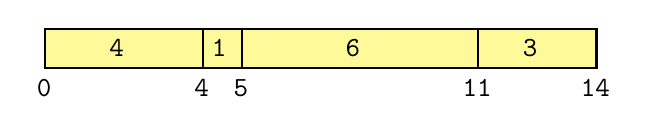
\begin{tikzpicture}[
	thick,
	font=\ttfamily\bfseries
]
\tikzset{
    myrect/.style = {rectangle, draw=black, align=center,anchor=west,fill=yellow!40,minimum height=0.5cm}
}
\node[myrect,minimum width=2.0cm] at (0,0) { 4 };
\node[myrect,minimum width=0.5cm] at (2,0) { 1 };
\node[myrect,minimum width=3.0cm] at (2.5,0) { 6 };
\node[myrect,minimum width=1.5cm] at (5.5,0) { 3 };
\node[] at (0,-0.50){0};
\node[] at (2,-0.50){4};
\node[] at (2.5,-0.50){5};
\node[] at (5.5,-0.50){11};
\node[] at (7,-0.50){14};
\end{tikzpicture}

Tempo di completamento medio:\\ $(4+5+11+14)/4 = 34/4 = 8.5$
\end{myboxtitle}


\pause
\begin{myboxtitle}[Shortest job first]
\medskip
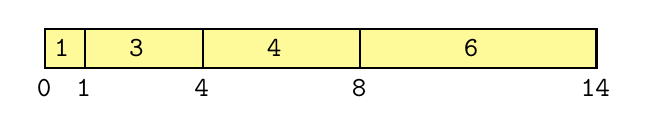
\begin{tikzpicture}[
	thick,
	font=\ttfamily\bfseries
]
\tikzset{
    myrect/.style = {rectangle, draw=black, align=center,anchor=west,fill=yellow!40,minimum height=0.5cm}
}
\node[myrect,minimum width=0.5cm] at (0.0,0) { 1 };
\node[myrect,minimum width=1.5cm] at (0.5,0) { 3 };
\node[myrect,minimum width=2.0cm] at (2.0,0) { 4 };
\node[myrect,minimum width=3.0cm] at (4.0,0) { 6 };
\node[] at (0.0,-0.50){0};
\node[] at (0.5,-0.50){1};
\node[] at (2.0,-0.50){4};
\node[] at (4.0,-0.50){8};
\node[] at (7,-0.50){14};
\end{tikzpicture}

Tempo di completamento medio:\\ $(1+4+8+14)/4 = 27/4 = 6.75$
\end{myboxtitle}

\end{frame}

%-------------------------------------------------------------------------
\begin{frame}{Dimostrazione di correttezza}


\vspace{-9pt}
\begin{myboxtitle}[Teorema - Scelta greedy]
Esiste una soluzione ottima $A$ in cui il job con minor tempo di fine $m$ si
trova in prima posizione ($A[1] = m)$.
\end{myboxtitle}

\begin{myboxtitle}[Teorema -- Sottostruttura ottima]
Sia $A$ una soluzione ottima di un problema con $n$ job, in cui il job
con minor tempo di fine $m$ si trova in prima posizione. La permutazione dei
seguenti $n-1$ job in $A$ è una soluzione ottima al sottoproblema in cui il
job $m$ non viene considerato.
\end{myboxtitle}

\end{frame}

%-------------------------------------------------------------------------
\begin{frame}{Dimostrazione -- Scelta greedy}

\vspace{-9pt}
\begin{myboxtitle}[Trasformazione soluzione ottima]
\BIL
\item Si consideri una permutazione ottima $A$:

\medskip
\IG{0.8}{sjf1-crop.pdf}

\item Sia \alert{$m$} la posizione in $A$  in cui si trova il job con \alert{minor tempo di fine}
\item Si consideri una permutazione $A'$ in cui i job in posizione $1$, $m$ vengono
scambiati: 

\medskip
\IG{0.8}{sjf2-crop.pdf}

\item Il tempo di completamento medio di $A'$ è minore o uguale al tempo di completamento medio di $A$
\EIL
\end{myboxtitle}
\end{frame}

%-------------------------------------------------------------------------
\begin{frame}{Dimostrazione -- Scelta greedy}

\vspace{-9pt}
\begin{myboxtitle}[La soluzione trasformata è anch'essa ottima]
\BIL

\item Il tempo di completamento medio di $A'$ è minore o uguale al tempo
di completamento medio di $A$
\medskip
\IG{0.8}{sjf3-crop.pdf}

  \BIL
	\item \color{red}{Job in posizione $1, \mydots, m-1$ in $A'$ hanno tempo di completamento $\leq$ dei job in posizione $1, \mydots, m-1$ in $A$}
	\item \color{blue}Job in posizione $m, \mydots, n$ in $A'$ hanno tempo di completamento $=$ dei job in posizione $m, \mydots, n$ in $A$
  \EIL
\item Poichè $A$ è ottima, $A'$ non può avere tempo di completamento medio minore e quindi anche $A'$ è ottima.
\EIL
\end{myboxtitle}
\end{frame}



%%%%%%%%%%%%%%%%%%%%%%%%%%%%%%%%%%%%%%%%%%%%%%%%%%%%%%%%%%%%%%%%%%%%%%%%%%
\section{Zaino frazionario}

%-------------------------------------------------------------------------
\begin{frame}{Problema dello zaino}

\vspace{-6pt}
\begin{myboxtitle}[Input]
\BIL
\item Un intero positivo $C$  - la capacità dello zaino
\item $n$ oggetti, tali che l'oggetto $i$-esimo è caratterizzato da
  \BI
	\item un profitto $p_i \in \mathbb{Z^+}$  
  \item un peso $w_i \in \mathbb{Z^+}$
	\EI
\EIL
\end{myboxtitle}

	
\begin{myboxtitle}[Zaino 0/1]
Trovare un sottoinsieme $S$ di $\{1, \mydots , n\}$ di oggetti tale che il loro
peso totale non superi la capacità massima e il loro profitto totale sia
massimo.
\end{myboxtitle}

\begin{myboxtitle}[Zaino reale (o Zaino frazionario)]
\EE possibile prendere frazioni di oggetti.
\end{myboxtitle}

\end{frame}

%-------------------------------------------------------------------------
\begin{frame}{Esempio}

\begin{overprint}
\onslide<1-2|handout:1>
\TwoCols{
  Consideriamo i tre oggetti a lato ed una capacità di 70
}{
\texttt{
\begin{tabular}{|r|r|r|}
\hline
\rowcolor{gray!20}
$i$ & $p_i$ & $w_i$ \\
\hline
\rowcolor{yellow!40} 1 & 60\$ & 10 \\
\hline
\rowcolor{blue!40} 2 & 200\$ & 40 \\
\hline
\rowcolor{red!20} 3 & 120\$ & 30 \\
\hline
\end{tabular}
}
}
\onslide<3|handout:2>
\TwoCols{
  Consideriamo i tre oggetti a lato ed una capacità di 70
}{
\texttt{
\begin{tabular}{|r|r|r|r|}
\hline
\rowcolor{gray!20}
$i$ & $p_i$ & $w_i$ & $p_i/w_i$ \\
\hline
\rowcolor{yellow!40} 1 & 60\$ & 10 & 6\$ \\
\hline
\rowcolor{blue!40} 2 & 200\$ & 40 & 5\$\\
\hline
\rowcolor{red!20} 3 & 120\$ & 30 & 4\$ \\
\hline
\end{tabular}
}
}
\end{overprint}

\bigskip
\begin{overprint}
\onslide<2|handout:1>
\BB{Approccio 1: Ordinati per \alert{profitto decrescente}}
\medskip
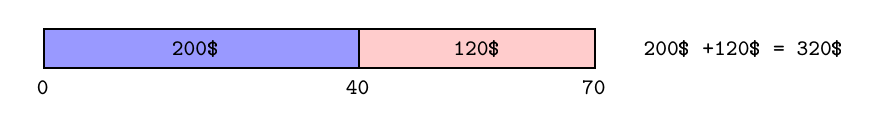
\begin{tikzpicture}[
	thick,
	font=\ttfamily\bfseries\footnotesize
]
\tikzset{
    myrect/.style = {rectangle, draw=black, align=center,anchor=west,fill=yellow!40,minimum height=0.5cm}
}
\node[myrect,minimum width=4.00cm,fill=blue!40] at (0.0,0) { 200\$ };
\node[myrect,minimum width=3.00cm,fill=red!20] at (4.0,0) { 120\$};
\node[align=left,anchor=west] at (7.5,0) {200\$ +120\$ = 320\$};
\node[] at (0.0,-0.50){0};
\node[] at (4.00,-0.50){40};
\node[] at (7.00,-0.50){70};
\end{tikzpicture}


\medskip
\BB{Approccio 2: Ordinati per \alert{peso crescente}}
\medskip
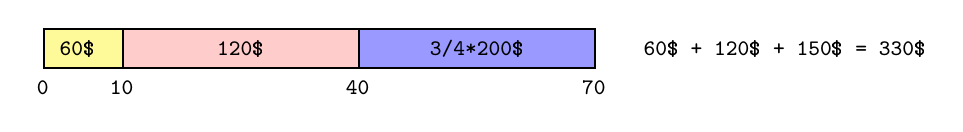
\begin{tikzpicture}[
	thick,
	font=\ttfamily\bfseries\footnotesize
]
\tikzset{
    myrect/.style = {rectangle, draw=black, align=center,anchor=west,fill=yellow!40,minimum height=0.5cm}
}
\node[myrect,minimum width=1.0cm,fill=yellow!40] at (0.0,0) { 60\$ };
\node[myrect,minimum width=3.0cm,fill=red!20] at (1.0,0) { 120\$};
\node[myrect,minimum width=3.0cm,fill=blue!40] at (4.0,0) { 3/4*200\$};
\node[align=left,anchor=west] at (7.5,0) {60\$ + 120\$ + 150\$ = 330\$};
\node[] at (0.0,-0.50){0};
\node[] at (1.0,-0.50){10};
\node[] at (4.0,-0.50){40};
\node[] at (7.0,-0.50){70};
\end{tikzpicture}

\onslide<3|handout:2>
\BB{Approccio 3: Ordinati per \alert{profitto specifico $p_i/w_i$ decrescente}}

\medskip
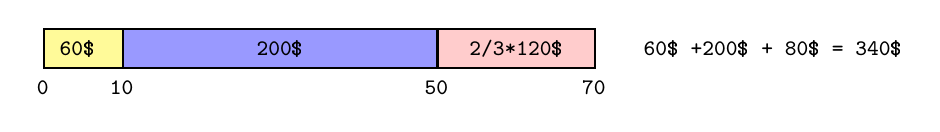
\begin{tikzpicture}[
	thick,
	font=\ttfamily\bfseries\footnotesize
]
\tikzset{
    myrect/.style = {rectangle, draw=black, align=center,anchor=west,fill=yellow!40,minimum height=0.5cm}
}
\node[myrect,minimum width=1.0cm,fill=yellow!40] at (0.0,0) { 60\$ };
\node[myrect,minimum width=4.0cm,fill=blue!40] at (1.0,0) { 200\$};
\node[myrect,minimum width=2.0cm,fill=red!20] at (5.0,0) { 2/3*120\$};
\node[align=left,anchor=west] at (7.5,0) {60\$ +200\$ + 80\$ = 340\$};
\node[] at (0.0,-0.50){0};
\node[] at (1.0,-0.50){10};
\node[] at (5.0,-0.50){50};
\node[] at (7.0,-0.50){70};
\end{tikzpicture}

\medskip
\BB{Approccio 3 non funziona per Zaino 0/1}

\medskip
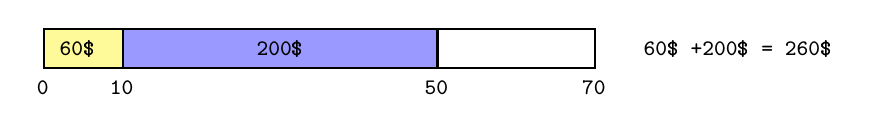
\begin{tikzpicture}[
	thick,
	font=\ttfamily\bfseries\footnotesize
]
\tikzset{
    myrect/.style = {rectangle, draw=black, align=center,anchor=west,fill=yellow!40,minimum height=0.5cm}
}
\node[myrect,minimum width=1.0cm,fill=yellow!40] at (0.0,0) { 60\$ };
\node[myrect,minimum width=4.0cm,fill=blue!40] at (1.0,0) { 200\$};
\node[myrect,minimum width=2.0cm,fill=white] at (5.0,0) {};
\node[align=left,anchor=west] at (7.5,0) {60\$ +200\$  = 260\$};
\node[] at (0.0,-0.50){0};
\node[] at (1.0,-0.50){10};
\node[] at (5.0,-0.50){50};
\node[] at (7.0,-0.50){70};
\end{tikzpicture}

\end{overprint}
\end{frame}

%-------------------------------------------------------------------------
\begin{frame}{Algoritmo}
\begin{Procedure}
\caption[A]{$\REAL[\,]$\ \zaino($\REAL[\,]\ p,\ \REAL[\,]\ w,\REAL\ C,\ \INTEGER\ n$)}
$\REAL[\,]\ x = \NEW\ \REAL[1 \mydots n]$\;
\{ ordina $p$ e $w$ in modo che $p[1]/w[1] \ge p[2]/w[2] \ge \cdots \ge p[n]/w[n]$\}\;
\For{$i=1$ \TO\ $n$}
{
  $x[i] = \MIN(C/w[i], 1)$\;
  $C = C - x[i] \cdot w[i]$\;
}
\Return $x$
\end{Procedure}

\makebox[2.5cm][l]{\alert{Complessità}:} $O(n \log n)$ se input non è ordinato\\
\makebox[2.5cm][l]{} $O(n)$ se l'input è già ordinato.

\bigskip
$x[i] \in [0,1]$ rappresenta la porzione dell'oggetto $i$-esimo
che deve essere prelevata.

\end{frame}

%-------------------------------------------------------------------------
\begin{frame}{Correttezza}

\BB{Informalmente}

\BIL
\item Assumiamo che gli oggetti siano ordinati per profitto specifico decrescente
\item Sia $x$ una soluzione ottima
\item Supponiamo che $x[1] < \MIN(C/w[i], 1) < 1$ 
\item Allora possiamo costruire una nuova soluzione in cui $x'[1] = \MIN(C/w[i], 1)$ e 
la proporzione di uno o più oggetti è ridotta di conseguenza
\item Otteniamo così una soluzione $x'$ di profitto uguale o superiore, visto
che il profitto specifico dell'oggetto $1$ è massimo
\EIL

\end{frame}

%%%%%%%%%%%%%%%%%%%%%%%%%%%%%%%%%%%%%%%%%%%%%%%%%%%%%%%%%%%%%%%%%%%%%%%%%%
\section{Compressione di Huffman}


%-------------------------------------------------------------------------
\begin{frame}{Problema della compressione}

\BB{Rappresentare i dati in modo efficiente}
\BIL
\item Impiegare il numero minore di bit per la rappresentazione
\item Obiettivo: risparmio spazio su disco e tempo di trasferimento
\EIL

\BB{Una possibile tecnica di compressione: \alert{codifica di caratteri}}
\BIL
\item Tramite \alert{funzione di codifica} $f: f(c) = x$
\BI
	\item $c$ è un possibile carattere preso da un alfabeto $\Sigma$
	\item $x$ è una rappresentazione binaria
	\item "$c$ è rappresentato da $x$"
\EI
\EIL
\end{frame}

%-------------------------------------------------------------------------
\begin{frame}{Possibili codifiche}

\vspace{-9pt}
\begin{myboxtitle}[Esempio]
\BI
\item Supponiamo di avere un file di $n$ caratteri
\item Composto da caratteri nell'alfabeto \texttt{abcdef}
\item Di cui conosciamo la frequenza relativa
\EI
\end{myboxtitle}

\bigskip
\begin{overprint}
\onslide<1|handout:1>
\begin{tabular}{|l|c|c|c|c|c|c|c|}
\hline
\textbf{Caratteri} & \texttt{a} & \texttt{b} & \texttt{c} & \texttt{d} & \texttt{e} & \texttt{f} & \textbf{Dim.} \\\hline
\textbf{Frequenza} & 45\% & 13\% & 12\% & 16\% & 9\% & 5\% & \\ \hline
\textbf{ASCII} & \texttt{\tiny 01100001} & \texttt{\tiny 01100010} & \texttt{\tiny 01100011} & \texttt{\tiny 01100100} & \texttt{\tiny 01100101} & \texttt{\tiny 01100110} & $8n$ \\\hline
\textbf{Codifica 1} & \texttt{\small 000} & \texttt{\small 001} & \texttt{\small 010} & \texttt{\small 011} & \texttt{\small 100} & \texttt{\small 101} & $3n$ \\\hline
\end{tabular}
\onslide<2|handout:2>
\begin{tabular}{|l|c|c|c|c|c|c|c|}
\hline
\textbf{Caratteri} & \texttt{a} & \texttt{b} & \texttt{c} & \texttt{d} & \texttt{e} & \texttt{f} & \textbf{Dim.} \\\hline
\textbf{Frequenza} & 45\% & 13\% & 12\% & 16\% & 9\% & 5\% & \\ \hline
\textbf{ASCII} & \texttt{\tiny 01100001} & \texttt{\tiny 01100010} & \texttt{\tiny 01100011} & \texttt{\tiny 01100100} & \texttt{\tiny 01100101} & \texttt{\tiny 01100110} & $8n$ \\\hline
\textbf{Codifica 1} & \texttt{\small 000} & \texttt{\small 001} & \texttt{\small 010} & \texttt{\small 011} & \texttt{\small 100} & \texttt{\small 101} & $3n$ \\\hline
\textbf{Codifica 2} & \texttt{\small 0} & \texttt{\small 101} & \texttt{\small 100} & \texttt{\small 111} & \texttt{\small 1101} & \texttt{\small 1100} & $2.24n$ \\\hline
\end{tabular}
\end{overprint}
\bigskip
\begin{overprint}
\onslide<1|handout:1>
\alert{Possiamo fare di meglio?}
\onslide<2|handout:2>
\alert{Costo totale}: $(0.45 \cdot 1+0.13 \cdot 3+0.12 \cdot 3+0.16 \cdot 3+0.09 \cdot 4+0.05 \cdot 4) \cdot n=2.24n$
\end{overprint}
\end{frame}

%-------------------------------------------------------------------------
\begin{frame}{Codifica a prefissi}

\vspace{-9pt}
\begin{myboxtitle}[Codice a prefisso]
In un codice a prefisso (meglio sarebbe "senza prefissi"), \alert{nessun codice è
prefisso di un altro codice} (condizione necessaria per la decodifica).
\end{myboxtitle}

\begin{myboxtitle}[Esempio 1]
\BI
\item Codice: "\texttt{a}" $\rightarrow$ \texttt{0}, "\texttt{b}" $\rightarrow$ \texttt{10}, "\texttt{c}" $\rightarrow$ \texttt{11}
\item "\texttt{babaca}": $\texttt{10} \cdot \texttt{0} \cdot \texttt{10} \cdot \texttt{0} \cdot \texttt{11} \cdot \texttt{0}$
\EI
\end{myboxtitle}

\begin{myboxtitle}[Esempio 2]
\BI
\item Codice: "\texttt{a}" $\rightarrow$ \texttt{0}, "\texttt{b}" $\rightarrow$ \texttt{1}, "\texttt{c}" $\rightarrow$ \texttt{11}
\item \texttt{111111}?
\EI
\end{myboxtitle}

\end{frame}


%-------------------------------------------------------------------------
\begin{frame}{Rappresentazione ad albero per la codifica}

\vspace{-9pt}
\begin{myboxtitle}[Alcune domande]
\BIL
\item \EE possibile che il testo codificato sia più lungo della rappresentazione con 3 bit?
\item Esistono testi "difficili" per questa codifica?
\item Come organizzare un algoritmo per la decodifica?
\EIL
\end{myboxtitle}

\begin{myboxtitle}[Cenni storici]
\BIL
\item David Huffman, 1952
\item Algoritmo ottimo per costruire codici prefissi
\item Oggi utilizzato come complemento di altri metodi di compressione
(e.g. in \texttt{pkzip}, \texttt{zip}, \texttt{winrar})
\EIL
\end{myboxtitle}

\end{frame}

%-------------------------------------------------------------------------
\begin{frame}{Rappresentazione ad albero per la decodifica}

\vspace{-12pt}
\TwoColsCustom{0.55}{0.40}{
\vspace{-6pt}
\begin{myboxtitle}[Alberi binari di decodifica]
\BI
\item Figlio sinistro/destro: $0$ / $1$
\item Caratteri dell'alfabeto sulle foglie
\EI
\end{myboxtitle}
\smallskip
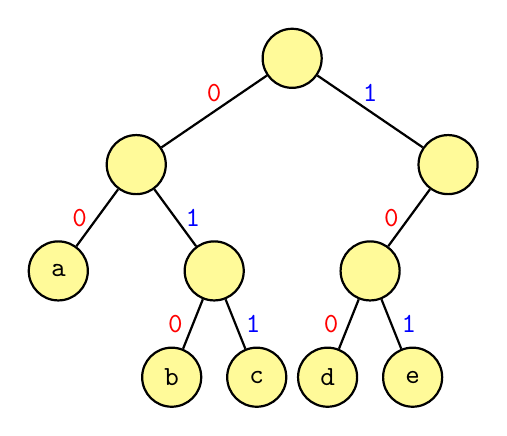
\begin{tikzpicture}[
	level distance=1.5cm,
  level 1/.style={sibling distance=4.4cm},
  level 2/.style={sibling distance=2.2cm},
  level 3/.style={sibling distance=1.2cm},
	thick,
	font=\ttfamily\bfseries,
    scale = 0.9
]
\tikzset{
    treenode/.style = {circle, draw=black, align=center,fill=yellow!40,minimum width=0.75cm},
		edgestyleL/.style = {midway,left,draw=none,text=red},
		edgestyleR/.style = {midway,right,draw=none,text=blue}
}
\node (root) [treenode] (T) {}
  child { node[treenode] (L) {} 
		child { node[treenode] (LL) {a} edge from parent node[edgestyleL] {0} }
  	child { node[treenode] (LR) {} 
			child { node[treenode] (LRL) {b} edge from parent node[edgestyleL] {0} }
  		child { node[treenode] (LRR) {c} edge from parent node[edgestyleR] {1} }
			edge from parent node[edgestyleR] {1}
		} 
		edge from parent node[edgestyleL,above] {0} 
	}
  child { node[treenode] (LR) {} 
		child { node[treenode](LRL) {} 
			child { node[treenode] {d} edge from parent node[edgestyleL] {0}}
  		child { node[treenode] {e} edge from parent node[edgestyleR] {1}}
			edge from parent node[edgestyleL] {0}
		}
  	child[missing] { node {}}
		edge from parent node[edgestyleR,above] {1}
	}
;	
\end{tikzpicture}
}{
\vspace{-6pt}
\begin{center}
\texttt{
\begin{tabular}{|c|c|c|c|c|}
\hline
a & b & c & d & e  \\\hline
\R{0}\R{0} & \R{0}\B{1}\R{0} & \R{0}\B{1}\B{1} & \B{1}\R{0}\R{0} & \B{1}\R{0}\B{1} \\\hline
\end{tabular}
}
\end{center}
{\small 
\begin{Procedure}
\caption[A]{Algoritmo di decodifica}
parti dalla radice\;
\While{file non è finito}{
	leggi un bit\;
	\eIf{bit è zero}{
 	 vai a sinistra\;
	 }{
  	vai a destra\;
		}
	\If{nodo foglia}{
  	stampa il carattere\;
		torna alla radice\;
	}
}
\end{Procedure}
}
}

\end{frame}

%-------------------------------------------------------------------------
\begin{frame}{Rappresentazione ad albero per la decodifica}

\vspace{-12pt}
\TwoColsCustom{0.55}{0.40}{
\vspace{-6pt}
\begin{myboxtitle}[Alberi binari di decodifica]
\BI
\item Figlio sinistro/destro: $0$ / $1$
\item Caratteri dell'alfabeto sulle foglie
\EI
\end{myboxtitle}
\smallskip
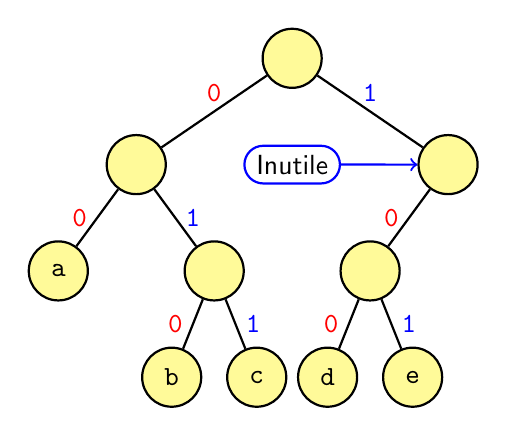
\begin{tikzpicture}[
	level distance=1.5cm,
  level 1/.style={sibling distance=4.4cm},
  level 2/.style={sibling distance=2.2cm},
  level 3/.style={sibling distance=1.2 cm},
	thick,
	font=\ttfamily\bfseries,
    scale = 0.9
]
\tikzset{
    treenode/.style = {circle, draw=black, align=center,fill=yellow!40,minimum width=0.75cm},
		edgestyleL/.style = {midway,left,draw=none,text=red},
		edgestyleR/.style = {midway,right,draw=none,text=blue}
}
\node (root) [treenode] (T) {}
  child { node[treenode] (L) {} 
		child { node[treenode] (LL) {a} edge from parent node[edgestyleL] {0} }
  	child { node[treenode] (LR) {} 
			child { node[treenode] (LRL) {b} edge from parent node[edgestyleL] {0} }
  		child { node[treenode] (LRR) {c} edge from parent node[edgestyleR] {1} }
			edge from parent node[edgestyleR] {1}
		} 
		edge from parent node[edgestyleL,above] {0} 
	}
  child { node[treenode] (R) {} 
		child { node[treenode](LRL) {} 
			child { node[treenode] {d} edge from parent node[edgestyleL] {0}}
  		child { node[treenode] {e} edge from parent node[edgestyleR] {1}}
			edge from parent node[edgestyleL] {0}
		}
  	child[missing] { node {}}
		edge from parent node[edgestyleR,above] {1}
	}
;	
\node[rounded rectangle,draw=blue,align=center,font=\sffamily] at (0, -1.5) (A) {Inutile};
\draw[->,blue] (A) to (R);
\end{tikzpicture}
}{
\vspace{-6pt}
\begin{center}
\texttt{
\begin{tabular}{|c|c|c|c|c|}
\hline
a & b & c & d & e  \\\hline
\R{0}\R{0} & \R{0}\B{1}\R{0} & \R{0}\B{1}\B{1} & \B{1}\R{0}\R{0} & \B{1}\R{0}\B{1} \\\hline
\end{tabular}
}
\end{center}
{\small 
\begin{Procedure}
\caption[A]{Algoritmo di decodifica}
parti dalla radice\;
\While{file non è finito}{
	leggi un bit\;
	\eIf{bit è zero}{
 	 vai a sinistra\;
	 }{
  	vai a destra\;
		}
	\If{nodo foglia}{
  	stampa il carattere\;
		torna alla radice\;
	}
}
\end{Procedure}
}
}

\end{frame}

%-------------------------------------------------------------------------
\begin{frame}{Rappresentazione ad albero per la decodifica}

\vspace{-12pt}
\TwoColsCustom{0.55}{0.40}{
\vspace{-6pt}
\begin{myboxtitle}[Alberi binari di decodifica]
\BI
\item Figlio sinistro/destro: $0$ / $1$
\item Caratteri dell'alfabeto sulle foglie
\EI
\end{myboxtitle}
\smallskip
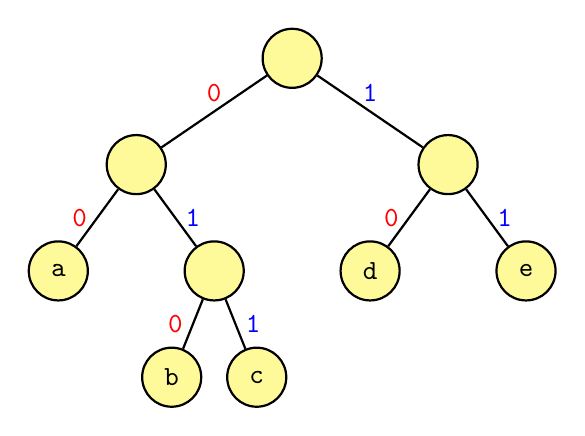
\begin{tikzpicture}[
	level distance=1.5cm,
  level 1/.style={sibling distance=4.4cm},
  level 2/.style={sibling distance=2.2cm},
  level 3/.style={sibling distance=1.2cm},
	thick,
	font=\ttfamily\bfseries, scale=0.9
]
\tikzset{
    treenode/.style = {circle, draw=black, align=center,fill=yellow!40,minimum width=0.75cm},
		edgestyleL/.style = {midway,left,draw=none,text=red},
		edgestyleR/.style = {midway,right,draw=none,text=blue}
}
\node [treenode] (T) {}
  child { node[treenode] (L) {} 
		child { node[treenode] (LL) {a} edge from parent node[edgestyleL] {0} }
  	child { node[treenode] (LR) {} 
			child { node[treenode] (LRL) {b} edge from parent node[edgestyleL] {0} }
  		child { node[treenode] (LRR) {c} edge from parent node[edgestyleR] {1} }
			edge from parent node[edgestyleR] {1}
		} 
		edge from parent node[edgestyleL,above] {0} 
	}
  child { node[treenode] (R) {} 
		child { node[treenode] {d} edge from parent node[edgestyleL] {0}}
  	child { node[treenode] {e} edge from parent node[edgestyleR] {1}}
		edge from parent node[edgestyleR,above] {1}
	}
;	
\end{tikzpicture}
}{
\vspace{-6pt}
\begin{center}
\texttt{
\begin{tabular}{|c|c|c|c|c|}
\hline
a & b & c & d & e  \\\hline
\R{0}\R{0} & \R{0}\B{1}\R{0} & \R{0}\B{1}\B{1} & \B{1}\R{0} & \B{1}\B{1} \\\hline
\end{tabular}
}
\end{center}
{\small 
\begin{Procedure}
\caption[A]{Algoritmo di decodifica}
parti dalla radice\;
\While{file non è finito}{
	leggi un bit\;
	\eIf{bit è zero}{
 	 vai a sinistra\;
	 }{
  	vai a destra\;
		}
	\If{nodo foglia}{
  	stampa il carattere\;
		torna alla radice\;
	}
}
\end{Procedure}
}
}

\end{frame}


%-------------------------------------------------------------------------
\begin{frame}{Definizione formale del problema}

\vspace{-9pt}
\begin{myboxtitle}[Input]
\BI
\item un file $F$ composto da caratteri nell'alfabeto $\Sigma$
\EI
\end{myboxtitle}

\begin{myboxtitle}[Quanti bit sono richiesti per codificare il file?]
\BI
\item Sia $T$ un albero che rappresenta la codifica
\item Per ogni $c \in \Sigma$, sia $d_T(c)$ la profondità della foglia che rappresenta c
\item Il codice per $c$ richiederà allora $d_T(c)$ bit
\item Se $f[c]$ è il numero di occorrenze di  $c$ in $F$, allora la dimensione della codifica è 
\[
  C(F,T) = \sum_{c \in \Sigma} f[c] \cdot d_T(c)
\]
\EI
\end{myboxtitle}

\end{frame}

%-------------------------------------------------------------------------
\begin{frame}{Algoritmo di Huffman}

\vspace{-9pt}
\begin{myboxtitle}[Principio del codice di Huffman]
\BIL
\item Minimizzare la lunghezza dei caratteri che compaiono più frequentemente
\item Assegnare ai caratteri con la frequenza minore i codici corrispondenti ai percorsi più lunghi all'interno dell'albero
\EIL
\end{myboxtitle}

\begin{myboxtitle}[Ogni codice è progettato per un file specifico]
\BIL
\item Si ottiene la frequenza di tutti i caratteri
\item Si costruisce il codice
\item Si rappresenta il file tramite il codice
\item Si aggiunge al file una rappresentazione del codice, per la decodifica
\EIL
\end{myboxtitle}

\end{frame}


%-------------------------------------------------------------------------
\begin{frame}[fragile]{Funzionamento algoritmo}

\vspace{-6pt}
\BB{
\BI
\item Costruire un nodo foglia per ogni carattere, etichettato con la propria frequenza
\EI
}

\medskip
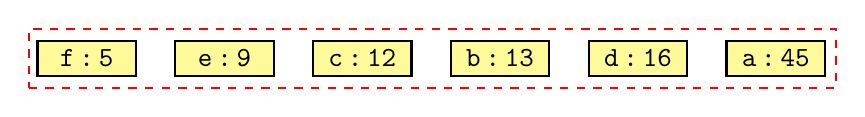
\begin{tikzpicture}[
	level distance=1.25cm,
  level 1/.style={sibling distance=1.75cm},
  level 2/.style={sibling distance=1.75cm},
  level 3/.style={sibling distance=1.75cm},
	thick,
	font=\ttfamily\bfseries
]
\tikzset{
    treenode/.style = {rectangle, draw=black, align=center,fill=yellow!40,minimum width=1.25cm},
}
\node[treenode] at (0.00,0) (A) {f\,:\,5};
\node[treenode] at (1.75,0) (B) {e\,:\,9};
\node[treenode] at (3.50,0) (C) {c\,:\,12};
\node[treenode] at (5.25,0) (D) {b\,:\,13};
\node[treenode] at (7.00,0) (E) {d\,:\,16};
\node[treenode] at (8.75,0) (F) {a\,:\,45};
\node[rectangle,anchor=west,minimum width=10.25cm,minimum height=0.75cm,dashed,draw=red] at (-0.75,0) {};
\end{tikzpicture}
\end{frame}


%-------------------------------------------------------------------------
\begin{frame}[fragile]{Funzionamento algoritmo}

\vspace{-6pt}
\BB{
\BI
\item Rimuovere i due nodi con frequenze minori $f_x$, $f_y$ 
\item Creare un nodo padre con etichetta "-" e frequenza $f_x+f_y$
\item Collegare i due nodi rimossi con il nuovo nodo
\item Aggiungere il nodo così creato all'insieme
\EI
}
\medskip
	
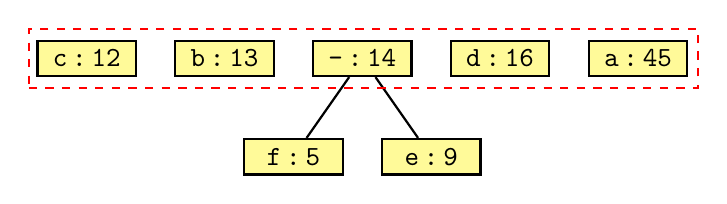
\begin{tikzpicture}[
	level distance=1.25cm,
  level 1/.style={sibling distance=1.75cm},
  level 2/.style={sibling distance=1.75cm},
  level 3/.style={sibling distance=1.75cm},
	thick,
	font=\ttfamily\bfseries
]
\tikzset{
    treenode/.style = {rectangle, draw=black, align=center,fill=yellow!40,minimum width=1.25cm},
}
\node[treenode] at (0.00,0) {c\,:\,12};
\node[treenode] at (1.75,0) {b\,:\,13};
\node[treenode] at (3.50,0) {-\,:\,14}
  child { node[treenode] {f\,:\,5} }
  child { node[treenode] {e\,:\,9} }
;
\node[treenode] at (5.25,0) {d\,:\,16};
\node[treenode] at (7.00,0) {a\,:\,45};
\node[rectangle,anchor=west,minimum width=8.5cm,minimum height=0.75cm,dashed,draw=red] at (-0.75,0) {};
\end{tikzpicture}
\end{frame}

%-------------------------------------------------------------------------
\begin{frame}[fragile]{Funzionamento algoritmo}

\vspace{-6pt}
\BB{
\BI
\item Rimuovere i due nodi con frequenze minori $f_x$, $f_y$ 
\item Creare un nodo padre con etichetta "-" e frequenza $f_x+f_y$
\item Collegare i due nodi rimossi con il nuovo nodo
\item Aggiungere il nodo così creato all'insieme
\EI
}
\medskip
	
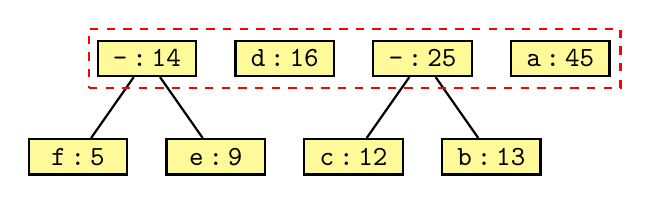
\begin{tikzpicture}[
	level distance=1.25cm,
  level 1/.style={sibling distance=1.75cm},
  level 2/.style={sibling distance=1.75cm},
  level 3/.style={sibling distance=1.75cm},
	thick,
	font=\ttfamily\bfseries
]
\tikzset{
    treenode/.style = {rectangle, draw=black, align=center,fill=yellow!40,minimum width=1.25cm},
}
\node[treenode] at (0.0,0) {-\,:\,14}
  child { node[treenode] {f\,:\,5} }
  child { node[treenode] {e\,:\,9} }
;
\node[treenode] at (1.75,0) {d\,:\,16};
\node[treenode] at (3.50,0) {-\,:\,25}
  child { node[treenode] {c\,:\,12} }
  child { node[treenode] {b\,:\,13} }
;
\node[treenode] at (5.25,0) {a\,:\,45};
\node[rectangle,anchor=west,minimum width=6.75cm,minimum height=0.75cm,dashed,draw=red] at (-0.75,0) {};
\end{tikzpicture}
\end{frame}

%-------------------------------------------------------------------------
\begin{frame}[fragile]{Funzionamento algoritmo}

\vspace{-6pt}
\BB{
\BI
\item Rimuovere i due nodi con frequenze minori $f_x$, $f_y$ 
\item Creare un nodo padre con etichetta "-" e frequenza $f_x+f_y$
\item Collegare i due nodi rimossi con il nuovo nodo
\item Aggiungere il nodo così creato all'insieme
\EI
}
\medskip
	
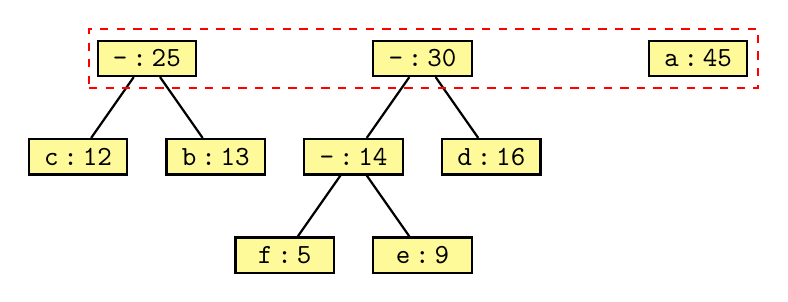
\begin{tikzpicture}[
	level distance=1.25cm,
  level 1/.style={sibling distance=1.75cm},
  level 2/.style={sibling distance=1.75cm},
  level 3/.style={sibling distance=1.75cm},
	thick,
	font=\ttfamily\bfseries
]
\tikzset{
    treenode/.style = {rectangle, draw=black, align=center,fill=yellow!40,minimum width=1.25cm},
}
\node[treenode] at (0.0,0) {-\,:\,25}
  child { node[treenode] {c\,:\,12} }
  child { node[treenode] {b\,:\,13} }
;
\node[treenode] at (3.5,0) {-\,:\,30}
  child { node[treenode] {-\,:\,14}
		child { node[treenode] {f\,:\,5} }
  	child { node[treenode] {e\,:\,9} }
	}
  child { node[treenode] {d\,:\,16} }
;
\node[treenode] at (7.0,0) {a\,:\,45};
\node[rectangle,anchor=west,minimum width=8.5cm,minimum height=0.75cm,dashed,draw=red] at (-0.75,0) {};
\end{tikzpicture}
\end{frame}


%-------------------------------------------------------------------------
\begin{frame}[fragile]{Funzionamento algoritmo}

\vspace{-6pt}
\BB{
\BI
\item Rimuovere i due nodi con frequenze minori $f_x$, $f_y$ 
\item Creare un nodo padre con etichetta "-" e frequenza $f_x+f_y$
\item Collegare i due nodi rimossi con il nuovo nodo
\item Aggiungere il nodo così creato all'insieme
\EI
}
\medskip
	
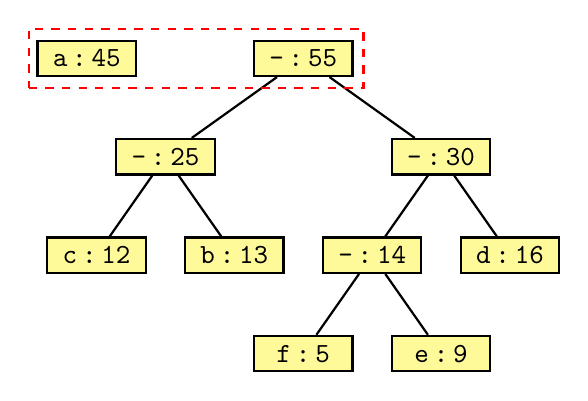
\begin{tikzpicture}[
	level distance=1.25cm,
  level 1/.style={sibling distance=3.50cm},
  level 2/.style={sibling distance=1.75cm},
  level 3/.style={sibling distance=1.75cm},
	thick,
	font=\ttfamily\bfseries
]
\tikzset{
    treenode/.style = {rectangle, draw=black, align=center,fill=yellow!40,minimum width=1.25cm},
}
\node[treenode] at (0.0,0) {a\,:\,45};
\node[treenode] at (2.75,0) {-\,:\,55}
child { node[treenode]  {-\,:\,25}
  child { node[treenode] {c\,:\,12} }
  child { node[treenode] {b\,:\,13} }
}
child { node[treenode]  {-\,:\,30}
  child { node[treenode] {-\,:\,14}
		child { node[treenode] {f\,:\,5} }
  	child { node[treenode] {e\,:\,9} }
	}
  child { node[treenode] {d\,:\,16} }
}
;
\node[rectangle,anchor=west,minimum width=4.25cm,minimum height=0.75cm,dashed,draw=red] at (-0.75,0) {};
\end{tikzpicture}
\end{frame}

%-------------------------------------------------------------------------
\begin{frame}[fragile]{Funzionamento algoritmo}

\vspace{-6pt}
\BB{
\BI
\item Si termina quando resta un solo nodo 
\EI
}
\medskip
	
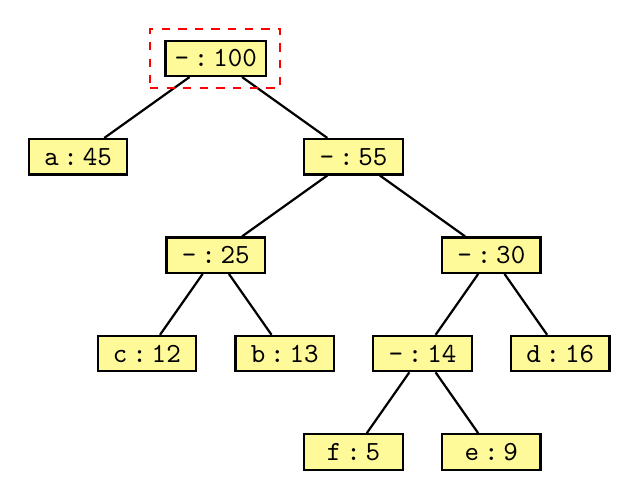
\begin{tikzpicture}[
	level distance=1.25cm,
  level 1/.style={sibling distance=3.5cm},
  level 2/.style={sibling distance=3.50cm},
  level 3/.style={sibling distance=1.75cm},
  level 4/.style={sibling distance=1.75cm},
	thick,
	font=\ttfamily\bfseries
]
\tikzset{
    treenode/.style = {rectangle, draw=black, align=center,fill=yellow!40,minimum width=1.25cm},
}
\node[treenode] at (0.0,0) {-\,:\,100}
child { node[treenode] {a\,:\,45} }
child { node[treenode] {-\,:\,55}
	child { node[treenode]  {-\,:\,25}
  	child { node[treenode] {c\,:\,12} }
  	child { node[treenode] {b\,:\,13} }
	}
	child { node[treenode]  {-\,:\,30}
  	child { node[treenode] {-\,:\,14}
			child { node[treenode] {f\,:\,5} }
  		child { node[treenode] {e\,:\,9} }
		}
  	child { node[treenode] {d\,:\,16} }
	}
}
;
\node[rectangle,anchor=west,minimum width=1.65cm,minimum height=0.75cm,dashed,draw=red] at (-0.85,0) {};
\end{tikzpicture}
\end{frame}

%-------------------------------------------------------------------------
\begin{frame}[fragile]{Funzionamento algoritmo}

\vspace{-6pt}
\BB{
\BI
\item Al termine, si etichettano gli archi dell'albero con bit \texttt{0},\texttt{1}
\EI

}
\medskip
	
\TwoColsCustom{0.7}{0.25}{
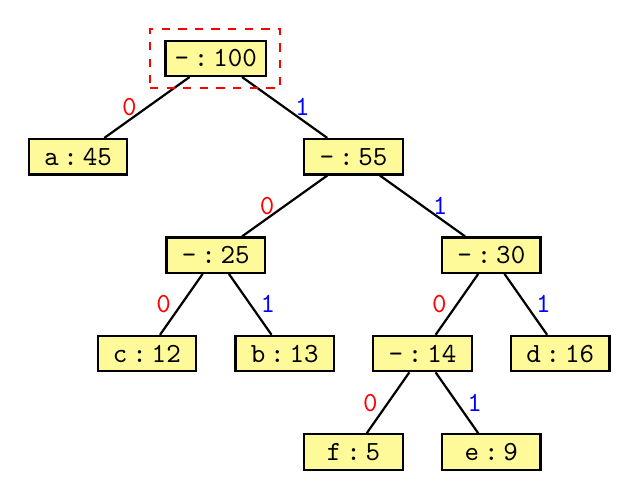
\begin{tikzpicture}[
	level distance=1.25cm,
  level 1/.style={sibling distance=3.5cm},
  level 2/.style={sibling distance=3.50cm},
  level 3/.style={sibling distance=1.75cm},
  level 4/.style={sibling distance=1.75cm},
	thick,
	font=\ttfamily\bfseries
]
\tikzset{
    treenode/.style = {rectangle, draw=black, align=center,fill=yellow!40,minimum width=1.25cm},
		edgestyleL/.style = {midway,left,draw=none,text=red},
		edgestyleR/.style = {midway,right,draw=none,text=blue}
}
\node[treenode] at (0.0,0) {-\,:\,100}
child { node[treenode] {a\,:\,45} edge from parent node[edgestyleL] {0} }
child { node[treenode] {-\,:\,55}
	child { node[treenode]  {-\,:\,25}
  	child { node[treenode] {c\,:\,12} edge from parent node[edgestyleL] {0} }
  	child { node[treenode] {b\,:\,13} edge from parent node[edgestyleR] {1}}
	edge from parent node[edgestyleL] {0} }
	child { node[treenode]  {-\,:\,30}
  	child { node[treenode] {-\,:\,14}
			child { node[treenode] {f\,:\,5} edge from parent node[edgestyleL] {0} }
  		child { node[treenode] {e\,:\,9} edge from parent node[edgestyleR] {1} }
			edge from parent node[edgestyleL] {0}
		}
  	child { node[treenode] {d\,:\,16} edge from parent node[edgestyleR] {1}}
	edge from parent node[edgestyleR] {1}	
	}
edge from parent node[edgestyleR] {1}
}
;
\node[rectangle,anchor=west,minimum width=1.65cm,minimum height=0.75cm,dashed,draw=red] at (-0.85,0) {};
\end{tikzpicture}
}{
\begin{center}
\texttt{
\begin{tabular}{|c|l|}
\hline
a & \R{0} \\\hline
b & \B{1}\R{0}\R{1} \\\hline
c & \B{1}\R{0}\B{0} \\\hline
d & \B{1}\B{1}\B{1} \\\hline
e & \B{1}\B{1}\R{0}\R{1} \\\hline
f & \B{1}\B{1}\R{0}\B{0} \\\hline
\end{tabular}
}
\end{center}
}
\end{frame}

%-------------------------------------------------------------------------
\begin{frame}{Algoritmo}

\TwoColsCustom{0.58}{0.41}{
\vspace{-18pt}
\begingroup
\small
\begin{Procedure}
\caption[A]{\Tree\ \fontproc{huffman}($\INTEGER[\,]\ c$, $\INTEGER[\,]\ f$, \INTEGER $n$)}

  $\Heap\ Q = \minheapconstructor()$\;
  \For{$i = 1$ \TO\ $n$}{
    $Q.\heapinsert(\treeconstructor(c[i], f[i]), f[i])$\;
  }
  \For{$i = 1$ \TO\ $n-1$}{
    $z_1 = Q.\heapdeletemin()$\;
    $z_2 = Q.\heapdeletemin()$\;
    $z = \treeconstructor(\Nil, z_1.f + z_2.f)$\;
    $z.\Leftvar = z_1$\;
    $z.\Rightvar = z_2$\;
    $Q.\heapinsert(z, z.f)$\;
  }
  \Return $Q.\heapdeletemin()$\;  
\end{Procedure}
\endgroup
}{

\vspace{-12pt}
\begin{myboxtitle}[Input]
\BI
\item[$n$]: numero caratteri
\item[$c \lbrack\,\rbrack$]: caratteri alfabeto
\item[$f \lbrack\,\rbrack$]: frequenze
\EI
\end{myboxtitle}

\begin{Procedure}
\caption[A]{\Tree}
  $c$ \Comment*{Carattere}
  $f$ \Comment*{Frequenza}
  $\mathit{left}$ \Comment*{Figlio sinistro}
  $\mathit{right}$ \Comment*{Figlio destro}
\end{Procedure}

\medskip
\alert{Complessità}: $O(n \log n)$
}
\end{frame}

%-------------------------------------------------------------------------
\begin{frame}{Correttezza}

\vspace{-9pt}
\begin{myboxtitle}[Teorema]
	L'output dell'algoritmo Huffman per un dato file è un codice a prefisso ottimo
\end{myboxtitle}

\begin{myboxtitle}[Proprietà della scelta greedy]
Scegliere i due elementi con la frequenza più bassa conduce sempre ad una soluzione ottimale
\end{myboxtitle}

\begin{myboxtitle}[Sottostruttura ottima]
Dato un problema sull'alfabeto $\Sigma$, è possibile costruire un sottoproblema con un alfabeto più piccolo
\end{myboxtitle}

\end{frame}


%-------------------------------------------------------------------------
\begin{frame}{Scelta greedy}

\vspace{-9pt}
\begin{myboxtitle}[Ipotesi]
\BI
\item Siano $\Sigma$ un alfabeto, $f$ un vettore di frequenze
\item Siano $x, y$ i \alert{due caratteri con frequenza più bassa}
\EI
\end{myboxtitle}

\begin{myboxtitle}[Tesi]
\BI
\item Esiste un codice prefisso ottimo per $\Sigma$ in cui $x,y$ hanno la stessa 
profondità massima e i loro codici differiscono solo per l'ultimo bit (sono foglie sorelle)
\EI
\end{myboxtitle}

\begin{myboxtitle}[Dimostrazione]
\BI
\item Al solito, basata sulla trasformazione di una soluzione ottima
\item Supponiamo che esista un codice ottimo $T$ in cui i due caratteri $a,b$ con profondità massima siano diversi da $x,y$
\EI
\end{myboxtitle}

\end{frame}

%-------------------------------------------------------------------------
\begin{frame}{Scelta greedy}

\vspace{-6pt}
\BIL
\item Assumiamo senza perdere di generalità: $f[x] \leq f[y]$,		$f[a] \leq f[b]$
\item Poiché le frequenze di $x$ e $y$ sono minime:    $f[x] \leq f[a]$,		$f[y] \leq f[b]$
\item Scambiamo $x$ con $a$: otteniamo $T'$
\item Scambiamo $y$ con $b$: otteniamo $T''$
\EIL

\medskip
\begin{columns}[T]
\column{0.32\linewidth}
\fbox{%
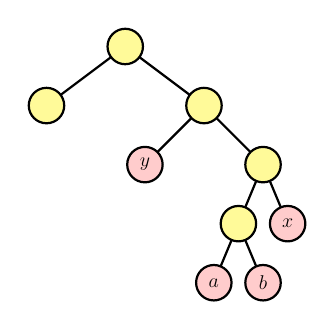
\begin{tikzpicture}[
    scale=0.5,
    transform shape,
	thick,
	level distance=1.5cm,
    level 1/.style={sibling distance=4cm}, 
    level 2/.style={sibling distance=3cm},
    level 3/.style={sibling distance=2cm},
    level 3/.style={sibling distance=1.25cm},
	font=\ttfamily\bfseries
  ]
  \node[mynode] {}
    child {node[mynode] {}
    }
    child {node[mynode] {}
      child {node[mynoder] {$y$}}
      child {node[mynode] {}
        child {node[mynode] {}
          child {node[mynoder] {$a$}}
          child {node[mynoder] {$b$}}
        }
        child {node[mynoder] {$x$}}
      }
    };
\end{tikzpicture}
}
\column{0.32\linewidth}
\fbox{%
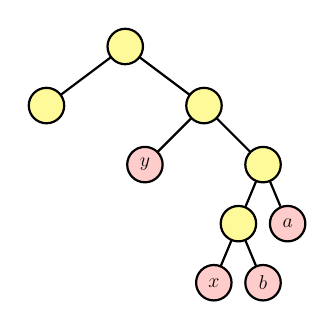
\begin{tikzpicture}[
    scale=0.5,
    transform shape,
	thick,
	level distance=1.5cm,
    level 1/.style={sibling distance=4cm}, 
    level 2/.style={sibling distance=3cm},
    level 3/.style={sibling distance=2cm},
    level 3/.style={sibling distance=1.25cm},
	font=\ttfamily\bfseries
  ]
  \node[mynode] {}
    child {node[mynode] {}
    }
    child {node[mynode] {}
      child {node[mynoder] {$y$}}
      child {node[mynode] {}
        child {node[mynode] {}
          child {node[mynoder] {$x$}}
          child {node[mynoder] {$b$}}
        }
        child {node[mynoder] {$a$}}
      }
    };
\end{tikzpicture}
}
\column{0.32\linewidth}
\fbox{%
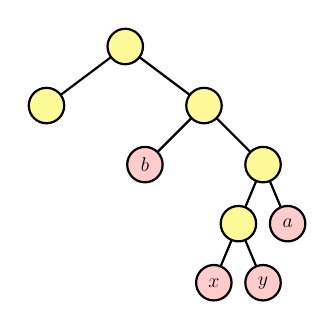
\begin{tikzpicture}[
    scale=0.5,
    transform shape,
	thick,
	level distance=1.5cm,
    level 1/.style={sibling distance=4cm}, 
    level 2/.style={sibling distance=3cm},
    level 3/.style={sibling distance=2cm},
    level 3/.style={sibling distance=1.25cm},
	font=\ttfamily\bfseries
  ]
  \node[mynode] {}
    child {node[mynode] {}
    }
    child {node[mynode] {}
      child {node[mynoder] {$b$}}
      child {node[mynode] {}
        child {node[mynode] {}
          child {node[mynoder] {$x$}}
          child {node[mynoder] {$y$}}
        }
        child {node[mynoder] {$a$}}
      }
    };
\end{tikzpicture}
}
\end{columns}

\end{frame}

%-------------------------------------------------------------------------
\begin{frame}[shrink=10]{Scelta greedy}

\BIL
\item Dimostriamo che: $C(f,T'') \leq C(f, T') \leq C(f,T)$

\begin{eqnarray*}
C(f,T) - C(f,T') &=& \sum_{c \in \Sigma} f[c]d_T(c) - \sum_{c \in \Sigma} f[c]d_{T'}(c) \\
             &=& (f[x]d_T(x)+f[a]d_T(a)) - (f[x]d_{T'}(x)+f[a]d_{T'}(a)) \\
             &=& (f[x]d_T(x)+f[a]d_T(a)) - (f[x]d_{T}(a)+f[a]d_{T}(x)) \\
             &=& (f[a]-f[x])(d_T(a)-d_T(x)) \\
             &\geq& 0 \\
C(f,T') - C(f,T'') &\geq& 0 \qquad \textrm{Come sopra}
\end{eqnarray*}

\item Ma poiché $T$ è ottimo, sappiamo anche che: $C(f,T) \leq C(f,T'')$
\item Quindi $T''$ è anch'esso ottimo
\EIL

\end{frame}

\begin{OnlySlides}{MC Microcomputer n.49 - Febbraio 1986}

\TwoCols{
\vspace{-21pt}
\IG{0.90}{mc049-huffman.pdf}
}{
Nelle pubblicità:
\BIL
\item Hard-disk 10MB per l'equivalente di 2400 Euro
%%% Proiettando, un'hard SSD da 1TB, che costa 160 euro nel 2019 su amazon, a questi prezzi viene 240 milioni di euro, una fattore 1.5 milioni
\item Mouse (con sfera) per l'equivalente di 200 Euro
\EIL

\IG{0.4}{huffman-david.jpg}
\vspace{-18pt}
\begin{center}
\tiny
\url{https://www.cise.ufl.edu/~manuel/huffman/press.release.html}
\end{center}
}

\end{OnlySlides}

\section{Alberi di copertura di peso minimo}

%-------------------------------------------------------------------------
\begin{frame}{Albero di copertura di peso minimo}

\vspace{-9pt}
\begin{myboxtitle}[Problema]
Dato un grafo pesato, determinare come interconnettere tutti i suoi nodi
minimizzando il costo del peso associato ai suoi archi.
\BI
\item \alert{Albero di copertura (di peso) minimo}
\item \alert{Albero di connessione (di peso) minimo}
\item \alert	{Minimum spanning tree}
\EI
\end{myboxtitle}

\begin{myboxtitle}[Esempio di applicazione]
Una compagnia di telecomunicazioni deve stendere una nuova rete
in un quartiere; deve seguire le connessioni esistenti (la rete stradale)
e ogni arco ha un costo associato distinto (costi di scavo, etc.)
\end{myboxtitle}
\end{frame}

%-------------------------------------------------------------------------
\begin{frame}{Definizione del problema}

\vspace{-9pt}
\begin{myboxtitle}[Input]
\BIL
\item \alert{$G=(V,E)$}: un grafo non orientato e connesso 
\item \alert{$w: V \times V \rightarrow \mathbb{R}$}: una funzione di peso (costo di connessione)
\BI
\item se $(u,v) \in E$, allora $w(u,v)$ è il peso dell'arco $(u,v)$
\item se $(u,v) \not\in E$, allora $w(u,v) = +\infty$
\EI
\item Poiché $G$ non è orientato, $w(u,v) = w(v,u)$
\EIL
\end{myboxtitle}
\bigskip	
\centering
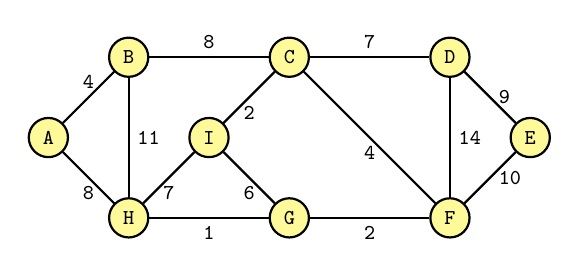
\begin{tikzpicture}[
	scale=0.85, 
	transform shape,
	thick,
	font=\ttfamily\bfseries\small
]
\tikzset{
    mynode/.style = {circle, draw=black, align=center,fill=yellow!40},
    edgen/.style = {-},
    edger/.style = {-,ultra thick,red}
}
\node[mynode] at (0.0,1.2) (a) {A};
\node[mynode] at (1.2,2.4) (b) {B};
\node[mynode] at (6.0,2.4) (d) {D};
\node[mynode] at (3.6,2.4) (c) {C};
\node[mynode] at (1.2,0.0) (h) {H};
\node[mynode] at (3.6,0.0) (g) {G};
\node[mynode] at (6.0,0.0) (f) {F};
\node[mynode] at (2.4,1.2) (i) {I};
\node[mynode] at (7.2,1.2) (e) {E};
%
\draw[edgen] (a) edge node[above] {4} (b);
\draw[edgen] (b) edge node[above] {8} (c);
\draw[edgen] (c) edge node[above] {7} (d);
\draw[edgen] (d) edge node[above,right] {9} (e);
%
\draw[edgen] (a) edge node[below] {8} (h);
\draw[edgen] (h) edge node[below] {1} (g);
\draw[edgen] (g) edge node[below] {2} (f);
\draw[edgen] (f) edge node[below,right] {10} (e);
%
\draw[edgen] (h) edge node[below] {7} (i);
\draw[edgen] (i) edge node[below] {6} (g);
\draw[edgen] (i) edge node[below] {2} (c);
%
\draw[edgen] (b) edge node[right] {11} (h);
\draw[edgen] (d) edge node[right] {14} (f);
\draw[edgen] (c) edge node[below] {4} (f);
\end{tikzpicture}

\end{frame}


%-------------------------------------------------------------------------
\begin{frame}{Definizione del problema}

\vspace{-9pt}
\begin{myboxtitle}[Albero di copertura (Spanning tree)]
Dato un grafo $G=(V,E)$ non orientato e connesso, un albero di copertura di $G$ è un sottografo $T=(V, E_T)$ 
tale che 
\BI
\item $T$ è un albero
\item $E_T \subseteq E$
\item $T$ contiene tutti i vertici di $G$
\EI
\end{myboxtitle}

\bigskip	
\centering
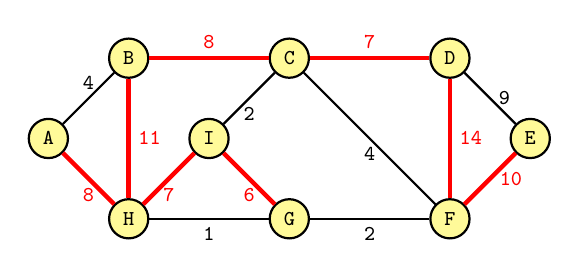
\begin{tikzpicture}[
	scale=0.85, 
	transform shape,
	thick,
	font=\ttfamily\bfseries\small
]
\tikzset{
    mynode/.style = {circle, draw=black, align=center,fill=yellow!40},
    edgen/.style = {-},
    edger/.style = {-,ultra thick,red}
}
\node[mynode] at (0.0,1.2) (a) {A};
\node[mynode] at (1.2,2.4) (b) {B};
\node[mynode] at (6.0,2.4) (d) {D};
\node[mynode] at (3.6,2.4) (c) {C};
\node[mynode] at (1.2,0.0) (h) {H};
\node[mynode] at (3.6,0.0) (g) {G};
\node[mynode] at (6.0,0.0) (f) {F};
\node[mynode] at (2.4,1.2) (i) {I};
\node[mynode] at (7.2,1.2) (e) {E};
%
\draw[edgen] (a) edge node[above] {4} (b);
\draw[edger] (b) edge node[above] {8} (c);
\draw[edger] (c) edge node[above] {7} (d);
\draw[edgen] (d) edge node[above,right] {9} (e);
%
\draw[edger] (a) edge node[below] {8} (h);
\draw[edgen] (h) edge node[below] {1} (g);
\draw[edgen] (g) edge node[below] {2} (f);
\draw[edger] (f) edge node[below,right] {10} (e);
%
\draw[edger] (h) edge node[below] {7} (i);
\draw[edger] (i) edge node[below] {6} (g);
\draw[edgen] (i) edge node[below] {2} (c);
%
\draw[edger] (b) edge node[right] {11} (h);
\draw[edger] (d) edge node[right] {14} (f);
\draw[edgen] (c) edge node[below] {4} (f);
\end{tikzpicture}

\end{frame}

%-------------------------------------------------------------------------
\begin{frame}{Definizione del problema}
\vspace{-6pt}
\begin{myboxtitle}[Output: albero di copertura di peso minimo]
Trovare l'albero di copertura il cui \alert{peso totale} sia minimo rispetto a ogni
altro albero di copertura.

\[
w(T) = \sum_{(u,v) \in E_T} w(u,v)
\]
\end{myboxtitle}

Non è detto che l'albero di copertura minimo sia univoco

\medskip
\centering
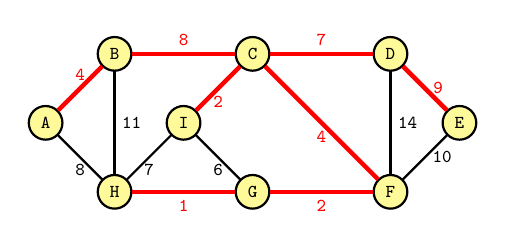
\begin{tikzpicture}[
	scale=0.73, 
	transform shape,
	thick,
	font=\ttfamily\bfseries\small
]
\tikzset{
    mynode/.style = {circle, draw=black, align=center,fill=yellow!40},
    edgen/.style = {-},
    edger/.style = {-,ultra thick,red}
}
\node[mynode] at (0.0,1.2) (a) {A};
\node[mynode] at (1.2,2.4) (b) {B};
\node[mynode] at (6.0,2.4) (d) {D};
\node[mynode] at (3.6,2.4) (c) {C};
\node[mynode] at (1.2,0.0) (h) {H};
\node[mynode] at (3.6,0.0) (g) {G};
\node[mynode] at (6.0,0.0) (f) {F};
\node[mynode] at (2.4,1.2) (i) {I};
\node[mynode] at (7.2,1.2) (e) {E};
%
\draw[edger] (a) edge node[above] {4} (b);
\draw[edger] (b) edge node[above] {8} (c);
\draw[edger] (c) edge node[above] {7} (d);
\draw[edger] (d) edge node[above,right] {9} (e);
%
\draw[edgen] (a) edge node[below] {8} (h);
\draw[edger] (h) edge node[below] {1} (g);
\draw[edger] (g) edge node[below] {2} (f);
\draw[edgen] (f) edge node[below,right] {10} (e);
%
\draw[edgen] (h) edge node[below] {7} (i);
\draw[edgen] (i) edge node[below] {6} (g);
\draw[edger] (i) edge node[below] {2} (c);
%
\draw[edgen] (b) edge node[right] {11} (h);
\draw[edgen] (d) edge node[right] {14} (f);
\draw[edger] (c) edge node[below] {4} (f);
\end{tikzpicture}
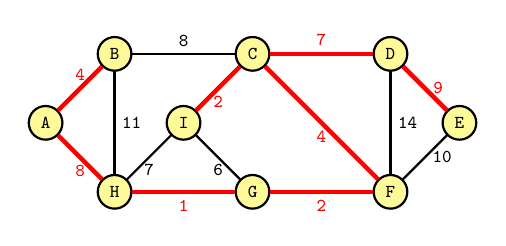
\begin{tikzpicture}[
	scale=0.73, 
	transform shape,
	thick,
	font=\ttfamily\bfseries\small
]
\tikzset{
    mynode/.style = {circle, draw=black, align=center,fill=yellow!40},
    edgen/.style = {-},
    edger/.style = {-,ultra thick,red}
}
\node[mynode] at (0.0,1.2) (a) {A};
\node[mynode] at (1.2,2.4) (b) {B};
\node[mynode] at (6.0,2.4) (d) {D};
\node[mynode] at (3.6,2.4) (c) {C};
\node[mynode] at (1.2,0.0) (h) {H};
\node[mynode] at (3.6,0.0) (g) {G};
\node[mynode] at (6.0,0.0) (f) {F};
\node[mynode] at (2.4,1.2) (i) {I};
\node[mynode] at (7.2,1.2) (e) {E};
%
\draw[edger] (a) edge node[above] {4} (b);
\draw[edgen] (b) edge node[above] {8} (c);
\draw[edger] (c) edge node[above] {7} (d);
\draw[edger] (d) edge node[above,right] {9} (e);
%
\draw[edger] (a) edge node[below] {8} (h);
\draw[edger] (h) edge node[below] {1} (g);
\draw[edger] (g) edge node[below] {2} (f);
\draw[edgen] (f) edge node[below,right] {10} (e);
%
\draw[edgen] (h) edge node[below] {7} (i);
\draw[edgen] (i) edge node[below] {6} (g);
\draw[edger] (i) edge node[below] {2} (c);
%
\draw[edgen] (b) edge node[right] {11} (h);
\draw[edgen] (d) edge node[right] {14} (f);
\draw[edger] (c) edge node[below] {4} (f);
\end{tikzpicture}

\end{frame}


\begin{frame}{Cammini minimi / alberi di copertura di peso minimo}

\vspace{-9pt}
\BB{Questi due alberi di copertura sono identici?}
\BI
\item un \alert<2>{albero dei cammini minimi} da singola sorgente $A$
\item un \alert<3>{albero di copertura di peso minimo}
\EI

\bigskip
\centering
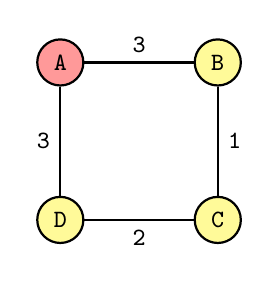
\begin{tikzpicture}[
    thick,
    font=\ttfamily\bfseries\small
]
\tikzset{
    mynode/.style = {circle, draw=black, align=center,fill=yellow!40},
    mynoder/.style = {circle, draw=black, align=center,fill=red!40},
    edgen/.style = {-},
    edger/.style = {-,ultra thick,red}
}
\node[mynode] at (0.0,0.0) (d) {D};
\node[mynoder] at (0.0,2.0) (a) {A};
\node[mynode] at (2.0,2.0) (b) {B};
\node[mynode] at (2.0,0.0) (c) {C};
\draw[edgen] (a) edge node[above] {3} (b);
\draw[edgen] (b) edge node[right] {1} (c);
\draw[edgen] (c) edge node[below] {2} (d);
\draw[edgen] (a) edge node[left] {3} (d);
\end{tikzpicture}
\qquad\pause
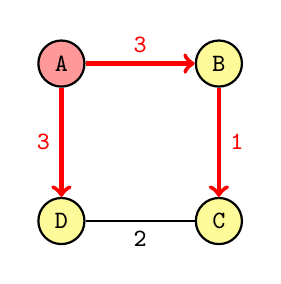
\begin{tikzpicture}[
    thick,
    font=\ttfamily\bfseries\small
]
\tikzset{
    mynode/.style = {circle, draw=black, align=center,fill=yellow!40},
    mynoder/.style = {circle, draw=black, align=center,fill=red!40},
    edgen/.style = {-},
    edger/.style = {->,ultra thick,red}
}
\node[mynode] at (0.0,0.0) (d) {D};
\node[mynoder] at (0.0,2.0) (a) {A};
\node[mynode] at (2.0,2.0) (b) {B};
\node[mynode] at (2.0,0.0) (c) {C};
\draw[edger] (a) edge node[above] {3} (b);
\draw[edger] (b) edge node[right] {1} (c);
\draw[edgen] (c) edge node[below] {2} (d);
\draw[edger] (a) edge node[left] {3} (d);
\end{tikzpicture}
\qquad\pause
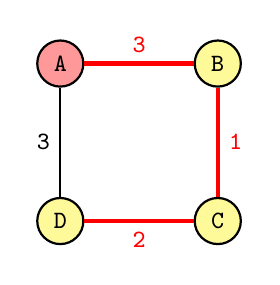
\begin{tikzpicture}[
    thick,
    font=\ttfamily\bfseries\small
]
\tikzset{
    mynode/.style = {circle, draw=black, align=center,fill=yellow!40},
    mynoder/.style = {circle, draw=black, align=center,fill=red!40},
    edgen/.style = {-},
    edger/.style = {-,ultra thick,red}
}
\node[mynode] at (0.0,0.0) (d) {D};
\node[mynoder] at (0.0,2.0) (a) {A};
\node[mynode] at (2.0,2.0) (b) {B};
\node[mynode] at (2.0,0.0) (c) {C};
\draw[edger] (a) edge node[above] {3} (b);
\draw[edger] (b) edge node[right] {1} (c);
\draw[edger] (c) edge node[below] {2} (d);
\draw[edgen] (d) edge node[left] {3} (a);
\end{tikzpicture}

\end{frame}


\begin{OnlySlides}{Città fangosa}
\begin{center}
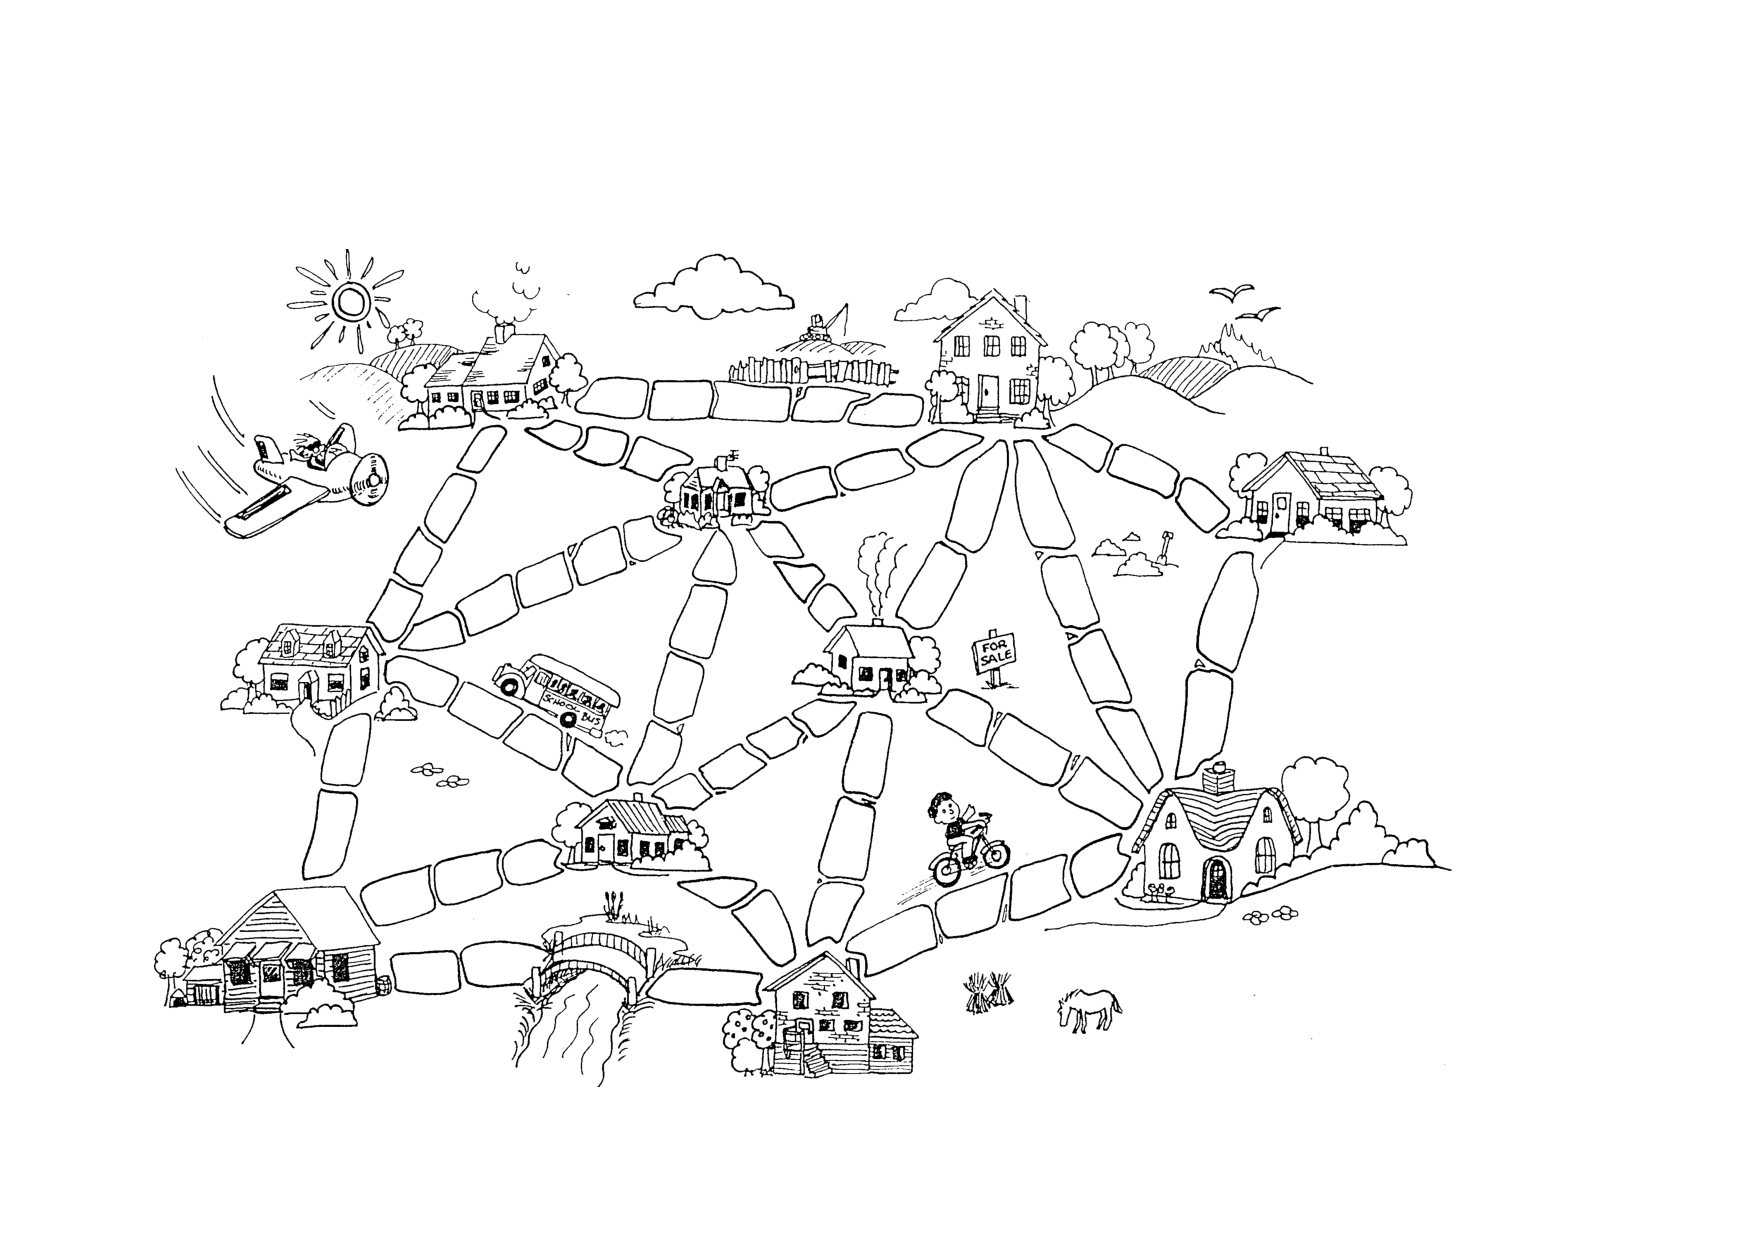
\includegraphics[width=\textwidth]{fangosa.pdf}
\end{center}
\end{OnlySlides}

%-------------------------------------------------------------------------
\begin{frame}{Algoritmo generico}

\vspace{-9pt}
\begin{myboxtitle}[Schema della lezione]
\BI
\item Progettiamo un algoritmo di tipo "ingordo" generico
\item Mostriamo due "istanze" di questo algoritmo: \alert{Kruskal} e \alert{Prim}
\EI
\end{myboxtitle}

\begin{myboxtitle}[Approccio]
L'idea è di accrescere un sottoinsieme $A$ di archi in modo tale che venga sempre
rispettata la seguente invariante:
\BI
\item $A$ è un sottoinsieme di qualche albero di connessione minimo
\EI
\end{myboxtitle}

\end{frame}

%-------------------------------------------------------------------------
\begin{frame}{Algoritmo generico}

\vspace{-9pt}
\begin{myboxtitle}[Arco sicuro]
Un arco $(u,v)$ è detto \alert{sicuro per $A$} se $A \cup \{(u,v)\}$ è ancora un sottoinsieme di qualche albero di connessione minimo.
\end{myboxtitle}

\medskip
\begin{Procedure}
\caption[A]{\Set\ \fontproc{mst-generico}(\Graph $G$, $\INTEGER[\,]\ w$)}

  \Set $A = \emptyset$\;
  \While{$A$ non forma un albero di copertura}
  {
     trova un arco sicuro $(u,v)$\;
     $A = A \cup \{(u,v)\}$\;
  } 
  \Return $A$\;  

\end{Procedure}

\end{frame}


%-------------------------------------------------------------------------
\begin{frame}{Definizioni}

\BI
\item Un \alert{taglio} $(S,V-S)$ di un grafo non orientato $G=(V,E)$ è una
partizione di $V$ in due sottoinsiemi disgiunti
\item Un arco $(u,v)$ \alert{attraversa} il taglio se $u \in S$ e $v \in V-S$
\item Un taglio \alert{rispetta} un insieme di archi $A$ se nessun arco di $A$
attraversa il taglio
\item Un arco che attraversa un taglio è \alert{leggero} nel taglio se il suo
peso è minimo fra i pesi degli archi che attraversano un taglio
\EI
\vspace{-12pt}
\centering
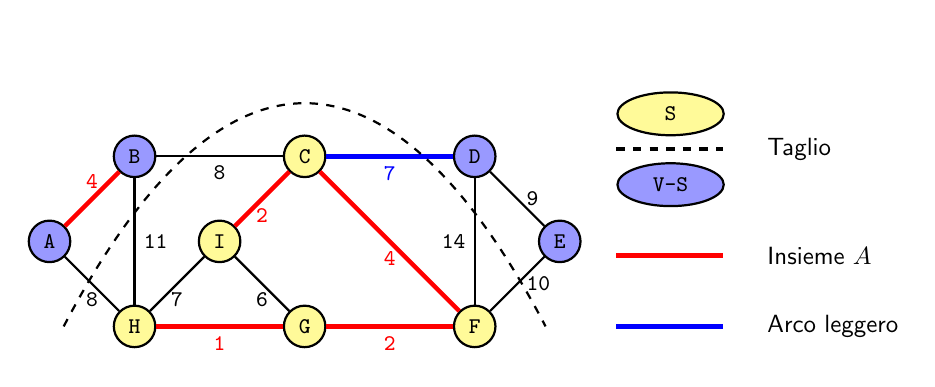
\begin{tikzpicture}[
	scale=0.9, 
	transform shape,
	thick,
	font=\ttfamily\bfseries\small
]
\tikzset{
    mynodea/.style = {circle, draw=black, align=center,fill=yellow!40},
    mynodeb/.style = {circle, draw=black, align=center,fill=blue!40},
    edgen/.style = {-},
    edger/.style = {-,ultra thick,red},
    edgeb/.style = {-,ultra thick,blue},
}
\node[mynodeb] at (0.0,1.2) (a) {A};
\node[mynodeb] at (1.2,2.4) (b) {B};
\node[mynodeb] at (6.0,2.4) (d) {D};
\node[mynodea] at (3.6,2.4) (c) {C};
\node[mynodea] at (1.2,0.0) (h) {H};
\node[mynodea] at (3.6,0.0) (g) {G};
\node[mynodea] at (6.0,0.0) (f) {F};
\node[mynodea] at (2.4,1.2) (i) {I};
\node[mynodeb] at (7.2,1.2) (e) {E};
%
\draw[edger] (a) edge node[above] {4} (b);
\draw[edgen] (b) edge node[below] {8} (c);
\draw[edgeb] (c) edge node[below] {7} (d);
\draw[edgen] (d) edge node[above,right] {9} (e);
%
\draw[edgen] (a) edge node[below] {8} (h);
\draw[edger] (h) edge node[below] {1} (g);
\draw[edger] (g) edge node[below] {2} (f);
\draw[edgen] (f) edge node[below,right] {10} (e);
%
\draw[edgen] (h) edge node[below] {7} (i);
\draw[edgen] (i) edge node[below] {6} (g);
\draw[edger] (i) edge node[below] {2} (c);
%
\draw[edgen] (b) edge node[right] {11} (h);
\draw[edgen] (d) edge node[left] {14} (f);
\draw[edger] (c) edge node[below] {4} (f);
\path[draw,dashed] (0.2,0) .. controls (2.4,4.2) and (4.8,4.2) .. (7.0,0);

\node[ellipse,draw=black, align=center,fill=yellow!40, minimum width=1.5cm,anchor=west] at (8,3.0) (e) {S};
\node[ellipse,draw=black, align=center,fill=blue!40, minimum width=1.5cm,anchor=west] at (8,2.0) (e) {V-S};
\node[font=\sffamily,anchor=west,align=left] at (10.0,2.5) {Taglio};
\node[font=\sffamily,anchor=west,align=left] at (10.0,1.0) {Insieme $A$};
\node[font=\sffamily,anchor=west,align=left] at (10.0,0.0) {Arco leggero};
\draw[ultra thick,black,dashed] (8.00,2.5) -- (9.5,2.5);
\draw[ultra thick,red] (8.00,1.0) -- (9.5,1.0);
\draw[ultra thick,blue] (8.00,0.0) -- (9.5,0.0);
\end{tikzpicture}

\end{frame}


%-------------------------------------------------------------------------
\begin{frame}{Arco sicuro}

\vspace{-9pt}
\begin{myboxtitle}[Teorema]
\BIL
\item Sia $G=(V,E)$ un grafo non orientato e connesso 
\item Sia $w: V \times V \rightarrow \mathbb{R}$
\item Sia $A \subseteq E$ un sottoinsieme contenuto in un qualche albero di copertura minimo per $G$ 
\item Sia $(S,V-S)$ un qualunque taglio che rispetta $A$
\item Sia $(u,v)$ un arco leggero che attraversa il taglio
\EIL

\bigskip
$\Rightarrow$ l'arco $(u,v)$ è sicuro per $A$	
\end{myboxtitle}
\end{frame}


%-------------------------------------------------------------------------
\begin{frame}{Esempio: arco non sicuro perché il taglio non rispetta A}

\vspace{-12pt}
\TwoColsCustom{0.25}{0.70}{
\vspace{24pt}
Arco blu sicuro
}{
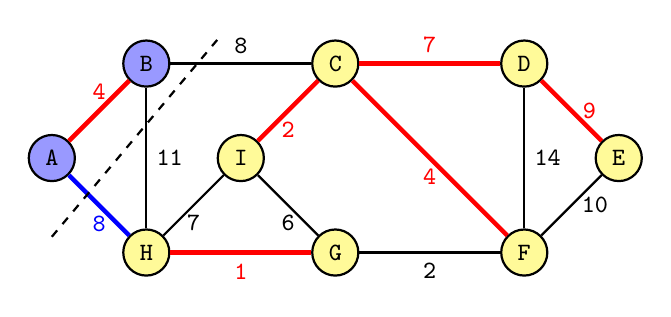
\begin{tikzpicture}[
	scale=1, 
	transform shape,
	thick,
	font=\ttfamily\bfseries\small
]
\tikzset{
    mynode/.style = {circle, draw=black, align=center,fill=yellow!40},
    mynodeb/.style = {circle, draw=black, align=center,fill=blue!40},
    edgen/.style = {-},
    edger/.style = {-,ultra thick,red},
    edgeb/.style = {-,ultra thick,blue}
}
\node[mynodeb] at (0.0,1.2) (a) {A};
\node[mynodeb] at (1.2,2.4) (b) {B};
\node[mynode] at (6.0,2.4) (d) {D};
\node[mynode] at (3.6,2.4) (c) {C};
\node[mynode] at (1.2,0.0) (h) {H};
\node[mynode] at (3.6,0.0) (g) {G};
\node[mynode] at (6.0,0.0) (f) {F};
\node[mynode] at (2.4,1.2) (i) {I};
\node[mynode] at (7.2,1.2) (e) {E};
%
\draw[edger] (a) edge node[above] {4} (b);
\draw[edgen] (b) edge node[above] {8} (c);
\draw[edger] (c) edge node[above] {7} (d);
\draw[edger] (d) edge node[above,right] {9} (e);
%
\draw[edgeb] (a) edge node[below] {8} (h);
\draw[edger] (h) edge node[below] {1} (g);
\draw[edgen] (g) edge node[below] {2} (f);
\draw[edgen] (f) edge node[below,right] {10} (e);
%
\draw[edgen] (h) edge node[below] {7} (i);
\draw[edgen] (i) edge node[below] {6} (g);
\draw[edger] (i) edge node[below] {2} (c);
%
\draw[edgen] (b) edge node[right] {11} (h);
\draw[edgen] (d) edge node[right] {14} (f);
\draw[edger] (c) edge node[below] {4} (f);
\path[draw,dashed] (0.0,0.2) -- (2.1,2.7);
\end{tikzpicture}
}

\bigskip
\TwoColsCustom{0.25}{0.70}{
\vspace{24pt}
Arco blu non sicuro
}{
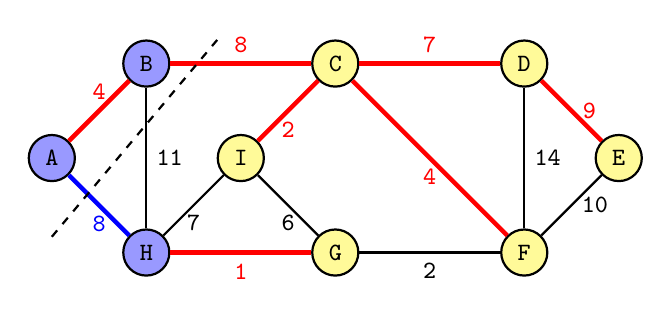
\begin{tikzpicture}[
	scale=1, 
	transform shape,
	thick,
	font=\ttfamily\bfseries\small
]
\tikzset{
    mynode/.style = {circle, draw=black, align=center,fill=yellow!40},
    mynodeb/.style = {circle, draw=black, align=center,fill=blue!40},
    edgen/.style = {-},
    edger/.style = {-,ultra thick,red},
    edgeb/.style = {-,ultra thick,blue}
}
\node[mynodeb] at (0.0,1.2) (a) {A};
\node[mynodeb] at (1.2,2.4) (b) {B};
\node[mynode] at (6.0,2.4) (d) {D};
\node[mynode] at (3.6,2.4) (c) {C};
\node[mynodeb] at (1.2,0.0) (h) {H};
\node[mynode] at (3.6,0.0) (g) {G};
\node[mynode] at (6.0,0.0) (f) {F};
\node[mynode] at (2.4,1.2) (i) {I};
\node[mynode] at (7.2,1.2) (e) {E};
%
\draw[edger] (a) edge node[above] {4} (b);
\draw[edger] (b) edge node[above] {8} (c);
\draw[edger] (c) edge node[above] {7} (d);
\draw[edger] (d) edge node[above,right] {9} (e);
%
\draw[edgeb] (a) edge node[below] {8} (h);
\draw[edger] (h) edge node[below] {1} (g);
\draw[edgen] (g) edge node[below] {2} (f);
\draw[edgen] (f) edge node[below,right] {10} (e);
%
\draw[edgen] (h) edge node[below] {7} (i);
\draw[edgen] (i) edge node[below] {6} (g);
\draw[edger] (i) edge node[below] {2} (c);
%
\draw[edgen] (b) edge node[right] {11} (h);
\draw[edgen] (d) edge node[right] {14} (f);
\draw[edger] (c) edge node[below] {4} (f);
\path[draw,dashed] (0.0,0.2) -- (2.1,2.7);
\end{tikzpicture}
}


\end{frame}

%-------------------------------------------------------------------------
\begin{frame}{Esempio: arco non sicuro perché non leggero}

\vspace{-12pt}
\TwoColsCustom{0.25}{0.70}{
\vspace{24pt}
Arco blu sicuro
}{
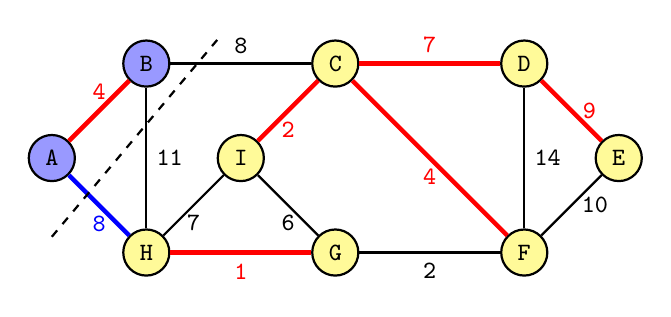
\begin{tikzpicture}[
	scale=1, 
	transform shape,
	thick,
	font=\ttfamily\bfseries\small
]
\tikzset{
    mynode/.style = {circle, draw=black, align=center,fill=yellow!40},
    mynodeb/.style = {circle, draw=black, align=center,fill=blue!40},
    edgen/.style = {-},
    edger/.style = {-,ultra thick,red},
    edgeb/.style = {-,ultra thick,blue}
}
\node[mynodeb] at (0.0,1.2) (a) {A};
\node[mynodeb] at (1.2,2.4) (b) {B};
\node[mynode] at (6.0,2.4) (d) {D};
\node[mynode] at (3.6,2.4) (c) {C};
\node[mynode] at (1.2,0.0) (h) {H};
\node[mynode] at (3.6,0.0) (g) {G};
\node[mynode] at (6.0,0.0) (f) {F};
\node[mynode] at (2.4,1.2) (i) {I};
\node[mynode] at (7.2,1.2) (e) {E};
%
\draw[edger] (a) edge node[above] {4} (b);
\draw[edgen] (b) edge node[above] {8} (c);
\draw[edger] (c) edge node[above] {7} (d);
\draw[edger] (d) edge node[above,right] {9} (e);
%
\draw[edgeb] (a) edge node[below] {8} (h);
\draw[edger] (h) edge node[below] {1} (g);
\draw[edgen] (g) edge node[below] {2} (f);
\draw[edgen] (f) edge node[below,right] {10} (e);
%
\draw[edgen] (h) edge node[below] {7} (i);
\draw[edgen] (i) edge node[below] {6} (g);
\draw[edger] (i) edge node[below] {2} (c);
%
\draw[edgen] (b) edge node[right] {11} (h);
\draw[edgen] (d) edge node[right] {14} (f);
\draw[edger] (c) edge node[below] {4} (f);
\path[draw,dashed] (0.0,0.2) -- (2.1,2.7);
\end{tikzpicture}
}

\bigskip
\TwoColsCustom{0.25}{0.70}{
\vspace{24pt}
Arco blu non sicuro
}{
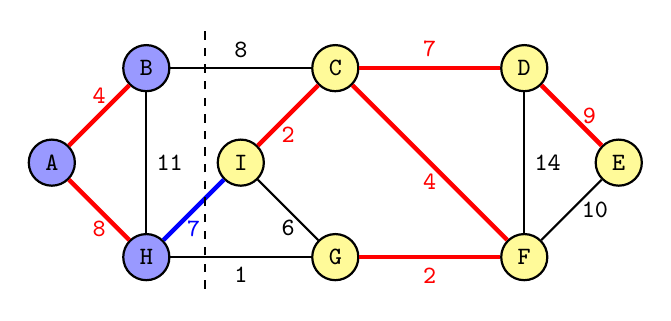
\begin{tikzpicture}[
	scale=1, 
	transform shape,
	thick,
	font=\ttfamily\bfseries\small
]
\tikzset{
    mynode/.style = {circle, draw=black, align=center,fill=yellow!40},
    mynodeb/.style = {circle, draw=black, align=center,fill=blue!40},
    edgen/.style = {-},
    edger/.style = {-,ultra thick,red},
    edgeb/.style = {-,ultra thick,blue}
}
\node[mynodeb] at (0.0,1.2) (a) {A};
\node[mynodeb] at (1.2,2.4) (b) {B};
\node[mynode] at (6.0,2.4) (d) {D};
\node[mynode] at (3.6,2.4) (c) {C};
\node[mynodeb] at (1.2,0.0) (h) {H};
\node[mynode] at (3.6,0.0) (g) {G};
\node[mynode] at (6.0,0.0) (f) {F};
\node[mynode] at (2.4,1.2) (i) {I};
\node[mynode] at (7.2,1.2) (e) {E};
%
\draw[edger] (a) edge node[above] {4} (b);
\draw[edgen] (b) edge node[above] {8} (c);
\draw[edger] (c) edge node[above] {7} (d);
\draw[edger] (d) edge node[above,right] {9} (e);
%
\draw[edger] (a) edge node[below] {8} (h);
\draw[edgen] (h) edge node[below] {1} (g);
\draw[edger] (g) edge node[below] {2} (f);
\draw[edgen] (f) edge node[below,right] {10} (e);
%
\draw[edgeb] (h) edge node[below] {7} (i);
\draw[edgen] (i) edge node[below] {6} (g);
\draw[edger] (i) edge node[below] {2} (c);
%
\draw[edgen] (b) edge node[right] {11} (h);
\draw[edgen] (d) edge node[right] {14} (f);
\draw[edger] (c) edge node[below] {4} (f);
%
\path[draw,dashed] (1.95,-0.4) -- (1.95, 2.9);
\end{tikzpicture}
}

\end{frame}


%-------------------------------------------------------------------------
\begin{frame}{Dimostrazione}

\vspace{-9pt}
\begin{myboxtitle}[Dimostrazione]
Sia $T$ un  albero di copertura minimo che contiene $A$. Due casi:
  \BI
	\item $(u,v) \in T$: allora $(u,v)$ è sicuro per $A$
	\item $(u,v) \not\in T$: trasformiamo $T$ in un albero $T'$ contenente
	  $(u,v)$ e dimostriamo che $T'$ è un albero di copertura minimo
	\EI
\end{myboxtitle}

\TwoColsCustom{0.75}{0.21}{
\BIL
\item $u,v$ sono connessi da un \alert{cammino} $C \subseteq T$\\ (per definizione di albero)
\item $u,v$ stanno in lati opposti del taglio\\ ($(u,v)$ attraversa il taglio)
\item $\exists (x,y) \in C$ che attraversa il taglio
\EIL
}{
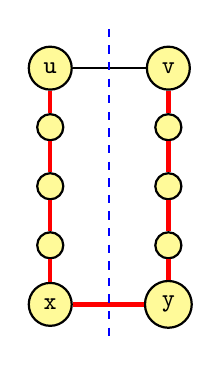
\begin{tikzpicture}[
	scale=1, 
	transform shape,
	thick,
	font=\ttfamily\bfseries\small
]
\tikzset{
    mynode/.style = {circle, draw=black, align=center,fill=yellow!40},
    edgen/.style = {-},
    edger/.style = {-,ultra thick,red},
}
\node[mynode] at (0.0,3.0) (u) {u};
\node[mynode] at (0.0,2.25) (u1) {};
\node[mynode] at (0.0,1.50) (u2) {};
\node[mynode] at (0.0,0.75) (u3) {};
\node[mynode] at (1.5,2.25) (v1) {};
\node[mynode] at (1.5,1.50) (v2) {};
\node[mynode] at (1.5,0.75) (v3) {};
\node[mynode] at (1.5,3.0) (v) {v};
\node[mynode] at (0.0,0.0) (x) {x};
\node[mynode] at (1.5,0.0) (y) {y};
\draw[edger] (x) to (y);
\draw[edger] (u) to (u1);
\draw[edger] (u1) to (u2);
\draw[edger] (u2) to (u3);
\draw[edger] (u3) to (x);
\draw[edger] (v) to (v1);
\draw[edger] (v1) to (v2);
\draw[edger] (v2) to (v3);
\draw[edger] (v3) to (y);
\draw[edgen] (u) to (v);
\path[draw,dashed,blue] (0.75,3.5) -- (0.75, -0.5);

\end{tikzpicture}
}
\end{frame}


%-------------------------------------------------------------------------
\begin{frame}{Dimostrazione}

\vspace{-9pt}
\begin{myboxtitle}[Dimostrazione]
Sia $T$ un  albero di copertura minimo che contiene $A$. Due casi
  \BI
	\item $(u,v) \in T$: allora $(u,v)$ è sicuro per $A$
	\item $(u,v) \not\in T$: trasformiamo $T$ in un albero $T'$ contenente
	  $(u,v)$ e dimostriamo che $T'$ è un albero di copertura minimo
	\EI
\end{myboxtitle}

\TwoColsCustom{0.75}{0.21}{
\BIL
\item $T' = T - \{ (x,y) \} \cup \{ (u,v) \}$
\item $T'$ è un albero di copertura
\item $w(T') \leq w(T)$ (perchè $w(u,v) \leq w(x,y)$)
\item $w(T) \leq w(T')$ (perchè $T$ minimo)
\EIL
}{
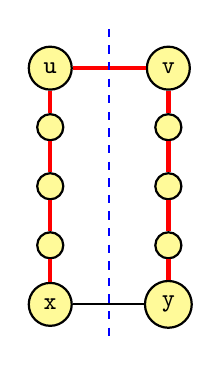
\begin{tikzpicture}[
	scale=1, 
	transform shape,
	thick,
	font=\ttfamily\bfseries\small
]
\tikzset{
    mynode/.style = {circle, draw=black, align=center,fill=yellow!40},
    edgen/.style = {-},
    edger/.style = {-,ultra thick,red},
}
\node[mynode] at (0.0,3.0) (u) {u};
\node[mynode] at (0.0,2.25) (u1) {};
\node[mynode] at (0.0,1.50) (u2) {};
\node[mynode] at (0.0,0.75) (u3) {};
\node[mynode] at (1.5,2.25) (v1) {};
\node[mynode] at (1.5,1.50) (v2) {};
\node[mynode] at (1.5,0.75) (v3) {};
\node[mynode] at (1.5,3.0) (v) {v};
\node[mynode] at (0.0,0.0) (x) {x};
\node[mynode] at (1.5,0.0) (y) {y};
\draw[edgen] (x) to (y);
\draw[edger] (u) to (u1);
\draw[edger] (u1) to (u2);
\draw[edger] (u2) to (u3);
\draw[edger] (u3) to (x);
\draw[edger] (v) to (v1);
\draw[edger] (v1) to (v2);
\draw[edger] (v2) to (v3);
\draw[edger] (v3) to (y);
\draw[edger] (u) to (v);
\path[draw,dashed,blue] (0.75,3.5) -- (0.75, -0.5);

\end{tikzpicture}

}


\end{frame}

%-------------------------------------------------------------------------
\begin{frame}{Archi sicuri}

\vspace{-9pt}
\begin{myboxtitle}[Corollario]
\BIL
\item Sia $G=(V,E)$ un grafo non orientato e connesso 
\item Sia $w: V \times V \rightarrow \mathbb{R}$
\item Sia $A \subseteq E$ un sottoinsieme contenuto in un qualche albero di copertura minimo per $G$ 
\item Sia $C$ una componente connessa (un albero) nella foresta $G_A=(V,A)$
\item Sia $(u,v)$ un arco leggero che connette $C$ a qualche altra componente in $G_A$
\EIL

\bigskip
$\Rightarrow$  l'arco $(u,v)$ è sicuro per $A$
\end{myboxtitle}

\end{frame}

%-------------------------------------------------------------------------
\begin{frame}{Algoritmo di Kruskal}

\vspace{-9pt}
\begin{myboxtitle}[Idea]
\BIL
\item Ingrandire sottoinsiemi disgiunti di un albero di copertura minimo
connettendoli fra di loro fino ad avere l’albero complessivo
\item Si individua un arco sicuro scegliendo un arco $(u,v)$ di peso minimo tra
tutti gli archi che connettono due distinti alberi (componenti connesse) della
foresta
\item L’algoritmo è greedy perché ad ogni passo si aggiunge alla foresta un
arco con il peso minore
\EIL
\end{myboxtitle}

\begin{myboxtitle}[Implementazione]
\BIL
\item Si utilizza una struttura dati Merge-Find Set
\EIL
\end{myboxtitle}

\end{frame}

%-------------------------------------------------------------------------
\begin{frame}{Algoritmo di Kruskal}
	
\vspace{-12pt}
\begin{Procedure}
\caption[A]{\Set\ \kruskal($\textsc{edge}[\,]\ A,\ \INTEGER\ n,\ \INTEGER\ m$)}

$\Set\ T = \setconstructor()$\;
$\mfset\ M = \mfconstructor(n)$\;
% $\Arco[\,]\ A = \new \Arco[1 \mldots G.m]$\;
% $\INTEGER\ i = 1$\;
% \ForEach{$u \in G.\VV$}{
%   \ForEach{$v \in G.\adj(u)$}{
%     $A[i] = \NEW\ \Arco$\;
%     $A[i].u = u; A[i.v]=v; A[i].\peso = w[u,v]$\;
%     $i = i+1$\;
%   }
% }
\{ ordina $A[1, \mldots, m]$ in modo che $A[1].\mathit{weight} \le \cdots \le A[m].\mathit{weight}$ \}\;
$\INTEGER\ \mathit{count} = 0$\;
$\INTEGER\ i = 1$\;
\textcolor{blue}{\% Termina quando l'albero ha $n-1$ archi o non ci sono più archi}\;
\While{$\mathit{count} < n-1$ \AND $i \leq m$}{
  \If{$M.\mffind(A[i].u) \neq M.\mffind(A[i].v)$}
  {
    $M.\mfmerge(A[i].u, A[i].v)$\;
    $T.\setinsert(A[i])$\;
    $\mathit{count} = \mathit{count}+1$\;
  }
  $i = i+1$\;	
}
\Return $T$\;
\end{Procedure}

\end{frame}

%-------------------------------------------------------------------------
\begin{frame}{Esempio}
	
%%%%%% 1 %%%%%%%%%%%%%%%%%
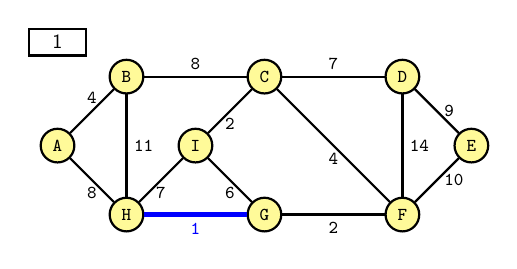
\begin{tikzpicture}[
	scale=0.73, 
	transform shape,
	thick,
	font=\ttfamily\bfseries\small
]
\tikzset{
    mynode/.style = {circle, draw=black, align=center,fill=yellow!40},
    edgen/.style = {-},
    edger/.style = {-,ultra thick,red},
    edgeb/.style = {-,ultra thick,blue}
}
\node[rectangle,draw=black,font=\sffamily, minimum width=1cm] at (0.0,3.0) {1};
\node[mynode] at (0.0,1.2) (a) {A};
\node[mynode] at (1.2,2.4) (b) {B};
\node[mynode] at (6.0,2.4) (d) {D};
\node[mynode] at (3.6,2.4) (c) {C};
\node[mynode] at (1.2,0.0) (h) {H};
\node[mynode] at (3.6,0.0) (g) {G};
\node[mynode] at (6.0,0.0) (f) {F};
\node[mynode] at (2.4,1.2) (i) {I};
\node[mynode] at (7.2,1.2) (e) {E};
%
\draw[edgen] (a) edge node[above] {4} (b);
\draw[edgen] (b) edge node[above] {8} (c);
\draw[edgen] (c) edge node[above] {7} (d);
\draw[edgen] (d) edge node[above,right] {9} (e);
%
\draw[edgen] (a) edge node[below] {8} (h);
\draw[edgeb] (h) edge node[below] {1} (g);
\draw[edgen] (g) edge node[below] {2} (f);
\draw[edgen] (f) edge node[below,right] {10} (e);
%
\draw[edgen] (h) edge node[below] {7} (i);
\draw[edgen] (i) edge node[below] {6} (g);
\draw[edgen] (i) edge node[below] {2} (c);
%
\draw[edgen] (b) edge node[right] {11} (h);
\draw[edgen] (d) edge node[right] {14} (f);
\draw[edgen] (c) edge node[below] {4} (f);
\end{tikzpicture}
\hfill
%%%%%% 2 %%%%%%%%%%%%%%%%%
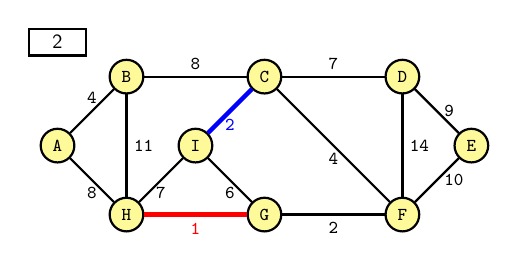
\begin{tikzpicture}[
	scale=0.73, 
	transform shape,
	thick,
	font=\ttfamily\bfseries\small
]
\tikzset{
    mynode/.style = {circle, draw=black, align=center,fill=yellow!40},
    edgen/.style = {-},
    edger/.style = {-,ultra thick,red},
    edgeb/.style = {-,ultra thick,blue}
}
\node[rectangle,draw=black,font=\sffamily, minimum width=1cm] at (0.0,3.0) {2};
\node[mynode] at (0.0,1.2) (a) {A};
\node[mynode] at (1.2,2.4) (b) {B};
\node[mynode] at (6.0,2.4) (d) {D};
\node[mynode] at (3.6,2.4) (c) {C};
\node[mynode] at (1.2,0.0) (h) {H};
\node[mynode] at (3.6,0.0) (g) {G};
\node[mynode] at (6.0,0.0) (f) {F};
\node[mynode] at (2.4,1.2) (i) {I};
\node[mynode] at (7.2,1.2) (e) {E};
%
\draw[edgen] (a) edge node[above] {4} (b);
\draw[edgen] (b) edge node[above] {8} (c);
\draw[edgen] (c) edge node[above] {7} (d);
\draw[edgen] (d) edge node[above,right] {9} (e);
%
\draw[edgen] (a) edge node[below] {8} (h);
\draw[edger] (h) edge node[below] {1} (g);
\draw[edgen] (g) edge node[below] {2} (f);
\draw[edgen] (f) edge node[below,right] {10} (e);
%
\draw[edgen] (h) edge node[below] {7} (i);
\draw[edgen] (i) edge node[below] {6} (g);
\draw[edgeb] (i) edge node[below] {2} (c);
%
\draw[edgen] (b) edge node[right] {11} (h);
\draw[edgen] (d) edge node[right] {14} (f);
\draw[edgen] (c) edge node[below] {4} (f);
\end{tikzpicture}

\bigskip
%%%%%% 3 %%%%%%%%%%%%%%%%%
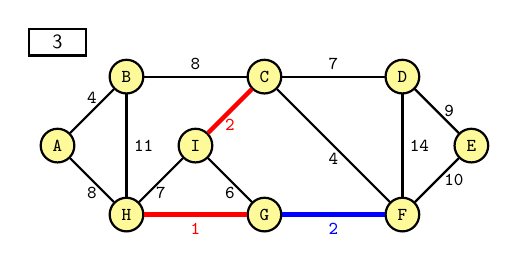
\begin{tikzpicture}[
	scale=0.73, 
	transform shape,
	thick,
	font=\ttfamily\bfseries\small
]
\tikzset{
    mynode/.style = {circle, draw=black, align=center,fill=yellow!40},
    edgen/.style = {-},
    edger/.style = {-,ultra thick,red},
    edgeb/.style = {-,ultra thick,blue}
}
\node[rectangle,draw=black,font=\sffamily, minimum width=1cm] at (0.0,3.0) {3};
\node[mynode] at (0.0,1.2) (a) {A};
\node[mynode] at (1.2,2.4) (b) {B};
\node[mynode] at (6.0,2.4) (d) {D};
\node[mynode] at (3.6,2.4) (c) {C};
\node[mynode] at (1.2,0.0) (h) {H};
\node[mynode] at (3.6,0.0) (g) {G};
\node[mynode] at (6.0,0.0) (f) {F};
\node[mynode] at (2.4,1.2) (i) {I};
\node[mynode] at (7.2,1.2) (e) {E};
%
\draw[edgen] (a) edge node[above] {4} (b);
\draw[edgen] (b) edge node[above] {8} (c);
\draw[edgen] (c) edge node[above] {7} (d);
\draw[edgen] (d) edge node[above,right] {9} (e);
%
\draw[edgen] (a) edge node[below] {8} (h);
\draw[edger] (h) edge node[below] {1} (g);
\draw[edgeb] (g) edge node[below] {2} (f);
\draw[edgen] (f) edge node[below,right] {10} (e);
%
\draw[edgen] (h) edge node[below] {7} (i);
\draw[edgen] (i) edge node[below] {6} (g);
\draw[edger] (i) edge node[below] {2} (c);
%
\draw[edgen] (b) edge node[right] {11} (h);
\draw[edgen] (d) edge node[right] {14} (f);
\draw[edgen] (c) edge node[below] {4} (f);
\end{tikzpicture}
\hfill
%%%%%% 4 %%%%%%%%%%%%%%%%%
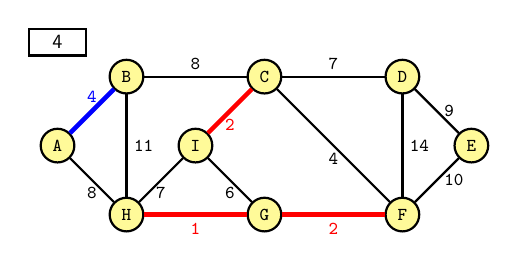
\begin{tikzpicture}[
	scale=0.73, 
	transform shape,
	thick,
	font=\ttfamily\bfseries\small
]
\tikzset{
    mynode/.style = {circle, draw=black, align=center,fill=yellow!40},
    edgen/.style = {-},
    edger/.style = {-,ultra thick,red},
    edgeb/.style = {-,ultra thick,blue}
}
\node[rectangle,draw=black,font=\sffamily, minimum width=1cm] at (0.0,3.0) {4};
\node[mynode] at (0.0,1.2) (a) {A};
\node[mynode] at (1.2,2.4) (b) {B};
\node[mynode] at (6.0,2.4) (d) {D};
\node[mynode] at (3.6,2.4) (c) {C};
\node[mynode] at (1.2,0.0) (h) {H};
\node[mynode] at (3.6,0.0) (g) {G};
\node[mynode] at (6.0,0.0) (f) {F};
\node[mynode] at (2.4,1.2) (i) {I};
\node[mynode] at (7.2,1.2) (e) {E};
%
\draw[edgeb] (a) edge node[above] {4} (b);
\draw[edgen] (b) edge node[above] {8} (c);
\draw[edgen] (c) edge node[above] {7} (d);
\draw[edgen] (d) edge node[above,right] {9} (e);
%
\draw[edgen] (a) edge node[below] {8} (h);
\draw[edger] (h) edge node[below] {1} (g);
\draw[edger] (g) edge node[below] {2} (f);
\draw[edgen] (f) edge node[below,right] {10} (e);
%
\draw[edgen] (h) edge node[below] {7} (i);
\draw[edgen] (i) edge node[below] {6} (g);
\draw[edger] (i) edge node[below] {2} (c);
%
\draw[edgen] (b) edge node[right] {11} (h);
\draw[edgen] (d) edge node[right] {14} (f);
\draw[edgen] (c) edge node[below] {4} (f);
\end{tikzpicture}
\end{frame}

%-------------------------------------------------------------------------
\begin{frame}{Esempio}
%%%%%% 5 %%%%%%%%%%%%%%%%%
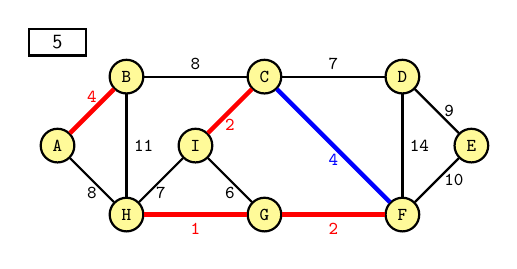
\begin{tikzpicture}[
	scale=0.73, 
	transform shape,
	thick,
	font=\ttfamily\bfseries\small
]
\tikzset{
    mynode/.style = {circle, draw=black, align=center,fill=yellow!40},
    edgen/.style = {-},
    edger/.style = {-,ultra thick,red},
    edgeb/.style = {-,ultra thick,blue}
}
\node[rectangle,draw=black,font=\sffamily, minimum width=1cm] at (0.0,3.0) {5};
\node[mynode] at (0.0,1.2) (a) {A};
\node[mynode] at (1.2,2.4) (b) {B};
\node[mynode] at (6.0,2.4) (d) {D};
\node[mynode] at (3.6,2.4) (c) {C};
\node[mynode] at (1.2,0.0) (h) {H};
\node[mynode] at (3.6,0.0) (g) {G};
\node[mynode] at (6.0,0.0) (f) {F};
\node[mynode] at (2.4,1.2) (i) {I};
\node[mynode] at (7.2,1.2) (e) {E};
%
\draw[edger] (a) edge node[above] {4} (b);
\draw[edgen] (b) edge node[above] {8} (c);
\draw[edgen] (c) edge node[above] {7} (d);
\draw[edgen] (d) edge node[above,right] {9} (e);
%
\draw[edgen] (a) edge node[below] {8} (h);
\draw[edger] (h) edge node[below] {1} (g);
\draw[edger] (g) edge node[below] {2} (f);
\draw[edgen] (f) edge node[below,right] {10} (e);
%
\draw[edgen] (h) edge node[below] {7} (i);
\draw[edgen] (i) edge node[below] {6} (g);
\draw[edger] (i) edge node[below] {2} (c);
%
\draw[edgen] (b) edge node[right] {11} (h);
\draw[edgen] (d) edge node[right] {14} (f);
\draw[edgeb] (c) edge node[below] {4} (f);
\end{tikzpicture}
\hfill
%%%%%% 6 %%%%%%%%%%%%%%%%%
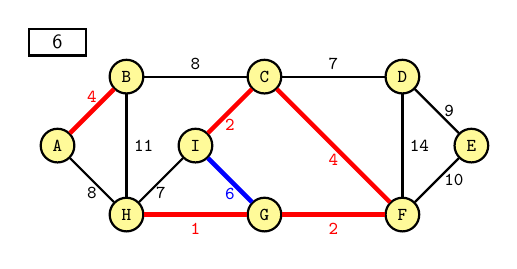
\begin{tikzpicture}[
	scale=0.73, 
	transform shape,
	thick,
	font=\ttfamily\bfseries\small
]
\tikzset{
    mynode/.style = {circle, draw=black, align=center,fill=yellow!40},
    edgen/.style = {-},
    edger/.style = {-,ultra thick,red},
    edgeb/.style = {-,ultra thick,blue}
}
\node[rectangle,draw=black,font=\sffamily, minimum width=1cm] at (0.0,3.0) {6};
\node[mynode] at (0.0,1.2) (a) {A};
\node[mynode] at (1.2,2.4) (b) {B};
\node[mynode] at (6.0,2.4) (d) {D};
\node[mynode] at (3.6,2.4) (c) {C};
\node[mynode] at (1.2,0.0) (h) {H};
\node[mynode] at (3.6,0.0) (g) {G};
\node[mynode] at (6.0,0.0) (f) {F};
\node[mynode] at (2.4,1.2) (i) {I};
\node[mynode] at (7.2,1.2) (e) {E};
%
\draw[edger] (a) edge node[above] {4} (b);
\draw[edgen] (b) edge node[above] {8} (c);
\draw[edgen] (c) edge node[above] {7} (d);
\draw[edgen] (d) edge node[above,right] {9} (e);
%
\draw[edgen] (a) edge node[below] {8} (h);
\draw[edger] (h) edge node[below] {1} (g);
\draw[edger] (g) edge node[below] {2} (f);
\draw[edgen] (f) edge node[below,right] {10} (e);
%
\draw[edgen] (h) edge node[below] {7} (i);
\draw[edgeb] (i) edge node[below] {6} (g);
\draw[edger] (i) edge node[below] {2} (c);
%
\draw[edgen] (b) edge node[right] {11} (h);
\draw[edgen] (d) edge node[right] {14} (f);
\draw[edger] (c) edge node[below] {4} (f);
\end{tikzpicture}	

\bigskip
%%%%%% 7 %%%%%%%%%%%%%%%%%
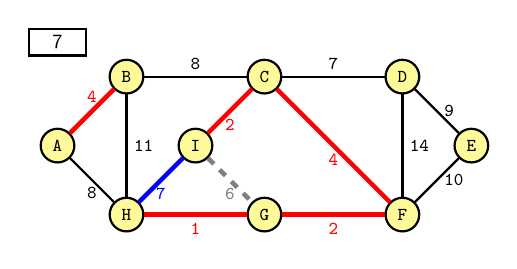
\begin{tikzpicture}[
	scale=0.73, 
	transform shape,
	thick,
	font=\ttfamily\bfseries\small
]
\tikzset{
    mynode/.style = {circle, draw=black, align=center,fill=yellow!40},
    edgen/.style = {-},
    edger/.style = {-,ultra thick,red},
    edgeb/.style = {-,ultra thick,blue},
    edgegg/.style = {-,ultra thick,gray,dashed},
}
\node[rectangle,draw=black,font=\sffamily, minimum width=1cm] at (0.0,3.0) {7};
\node[mynode] at (0.0,1.2) (a) {A};
\node[mynode] at (1.2,2.4) (b) {B};
\node[mynode] at (6.0,2.4) (d) {D};
\node[mynode] at (3.6,2.4) (c) {C};
\node[mynode] at (1.2,0.0) (h) {H};
\node[mynode] at (3.6,0.0) (g) {G};
\node[mynode] at (6.0,0.0) (f) {F};
\node[mynode] at (2.4,1.2) (i) {I};
\node[mynode] at (7.2,1.2) (e) {E};
%
\draw[edger] (a) edge node[above] {4} (b);
\draw[edgen] (b) edge node[above] {8} (c);
\draw[edgen] (c) edge node[above] {7} (d);
\draw[edgen] (d) edge node[above,right] {9} (e);
%
\draw[edgen] (a) edge node[below] {8} (h);
\draw[edger] (h) edge node[below] {1} (g);
\draw[edger] (g) edge node[below] {2} (f);
\draw[edgen] (f) edge node[below,right] {10} (e);
%
\draw[edgeb] (h) edge node[below] {7} (i);
\draw[edgegg] (i) edge node[below] {6} (g);
\draw[edger] (i) edge node[below] {2} (c);
%
\draw[edgen] (b) edge node[right] {11} (h);
\draw[edgen] (d) edge node[right] {14} (f);
\draw[edger] (c) edge node[below] {4} (f);
\end{tikzpicture}	
\hfill
%%%%%% 8 %%%%%%%%%%%%%%%%%
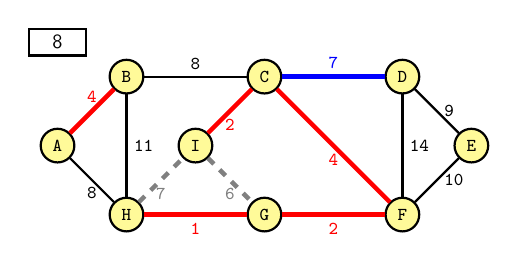
\begin{tikzpicture}[
	scale=0.73, 
	transform shape,
	thick,
	font=\ttfamily\bfseries\small
]
\tikzset{
    mynode/.style = {circle, draw=black, align=center,fill=yellow!40},
    edgen/.style = {-},
    edger/.style = {-,ultra thick,red},
    edgeb/.style = {-,ultra thick,blue},
    edgegg/.style = {-,ultra thick,gray,dashed},
}
\node[rectangle,draw=black,font=\sffamily, minimum width=1cm] at (0.0,3.0) {8};
\node[mynode] at (0.0,1.2) (a) {A};
\node[mynode] at (1.2,2.4) (b) {B};
\node[mynode] at (6.0,2.4) (d) {D};
\node[mynode] at (3.6,2.4) (c) {C};
\node[mynode] at (1.2,0.0) (h) {H};
\node[mynode] at (3.6,0.0) (g) {G};
\node[mynode] at (6.0,0.0) (f) {F};
\node[mynode] at (2.4,1.2) (i) {I};
\node[mynode] at (7.2,1.2) (e) {E};
%
\draw[edger] (a) edge node[above] {4} (b);
\draw[edgen] (b) edge node[above] {8} (c);
\draw[edgeb] (c) edge node[above] {7} (d);
\draw[edgen] (d) edge node[above,right] {9} (e);
%
\draw[edgen] (a) edge node[below] {8} (h);
\draw[edger] (h) edge node[below] {1} (g);
\draw[edger] (g) edge node[below] {2} (f);
\draw[edgen] (f) edge node[below,right] {10} (e);
%
\draw[edgegg] (h) edge node[below] {7} (i);
\draw[edgegg] (i) edge node[below] {6} (g);
\draw[edger] (i) edge node[below] {2} (c);
%
\draw[edgen] (b) edge node[right] {11} (h);
\draw[edgen] (d) edge node[right] {14} (f);
\draw[edger] (c) edge node[below] {4} (f);
\end{tikzpicture}	



\end{frame}


%-------------------------------------------------------------------------
\begin{frame}{Esempio}

%%%%%% 9 %%%%%%%%%%%%%%%%%
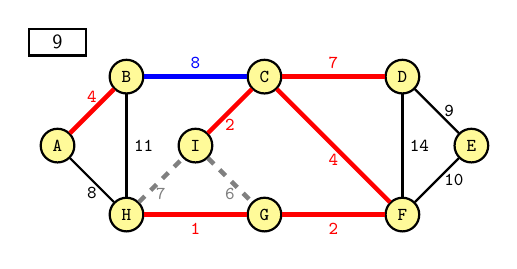
\begin{tikzpicture}[
	scale=0.73, 
	transform shape,
	thick,
	font=\ttfamily\bfseries\small
]
\tikzset{
    mynode/.style = {circle, draw=black, align=center,fill=yellow!40},
    edgen/.style = {-},
    edger/.style = {-,ultra thick,red},
    edgeb/.style = {-,ultra thick,blue},
    edgegg/.style = {-,ultra thick,gray,dashed},
}
\node[rectangle,draw=black,font=\sffamily, minimum width=1cm] at (0.0,3.0) {9};
\node[mynode] at (0.0,1.2) (a) {A};
\node[mynode] at (1.2,2.4) (b) {B};
\node[mynode] at (6.0,2.4) (d) {D};
\node[mynode] at (3.6,2.4) (c) {C};
\node[mynode] at (1.2,0.0) (h) {H};
\node[mynode] at (3.6,0.0) (g) {G};
\node[mynode] at (6.0,0.0) (f) {F};
\node[mynode] at (2.4,1.2) (i) {I};
\node[mynode] at (7.2,1.2) (e) {E};
%
\draw[edger] (a) edge node[above] {4} (b);
\draw[edgeb] (b) edge node[above] {8} (c);
\draw[edger] (c) edge node[above] {7} (d);
\draw[edgen] (d) edge node[above,right] {9} (e);
%
\draw[edgen] (a) edge node[below] {8} (h);
\draw[edger] (h) edge node[below] {1} (g);
\draw[edger] (g) edge node[below] {2} (f);
\draw[edgen] (f) edge node[below,right] {10} (e);
%
\draw[edgegg] (h) edge node[below] {7} (i);
\draw[edgegg] (i) edge node[below] {6} (g);
\draw[edger] (i) edge node[below] {2} (c);
%
\draw[edgen] (b) edge node[right] {11} (h);
\draw[edgen] (d) edge node[right] {14} (f);
\draw[edger] (c) edge node[below] {4} (f);
\end{tikzpicture}	
\hfill
%%%%%% 10 %%%%%%%%%%%%%%%%%
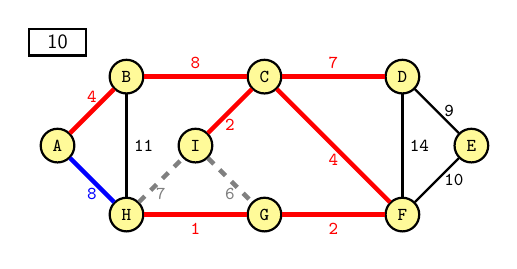
\begin{tikzpicture}[
	scale=0.73, 
	transform shape,
	thick,
	font=\ttfamily\bfseries\small
]
\tikzset{
    mynode/.style = {circle, draw=black, align=center,fill=yellow!40},
    edgen/.style = {-},
    edger/.style = {-,ultra thick,red},
    edgeb/.style = {-,ultra thick,blue},
    edgegg/.style = {-,ultra thick,gray,dashed},
}
\node[rectangle,draw=black,font=\sffamily, minimum width=1cm] at (0.0,3.0) {10};
\node[mynode] at (0.0,1.2) (a) {A};
\node[mynode] at (1.2,2.4) (b) {B};
\node[mynode] at (6.0,2.4) (d) {D};
\node[mynode] at (3.6,2.4) (c) {C};
\node[mynode] at (1.2,0.0) (h) {H};
\node[mynode] at (3.6,0.0) (g) {G};
\node[mynode] at (6.0,0.0) (f) {F};
\node[mynode] at (2.4,1.2) (i) {I};
\node[mynode] at (7.2,1.2) (e) {E};
%
\draw[edger] (a) edge node[above] {4} (b);
\draw[edger] (b) edge node[above] {8} (c);
\draw[edger] (c) edge node[above] {7} (d);
\draw[edgen] (d) edge node[above,right] {9} (e);
%
\draw[edgeb] (a) edge node[below] {8} (h);
\draw[edger] (h) edge node[below] {1} (g);
\draw[edger] (g) edge node[below] {2} (f);
\draw[edgen] (f) edge node[below,right] {10} (e);
%
\draw[edgegg] (h) edge node[below] {7} (i);
\draw[edgegg] (i) edge node[below] {6} (g);
\draw[edger] (i) edge node[below] {2} (c);
%
\draw[edgen] (b) edge node[right] {11} (h);
\draw[edgen] (d) edge node[right] {14} (f);
\draw[edger] (c) edge node[below] {4} (f);
\end{tikzpicture}	

\bigskip
\hfill
%%%%%% 11 %%%%%%%%%%%%%%%%%
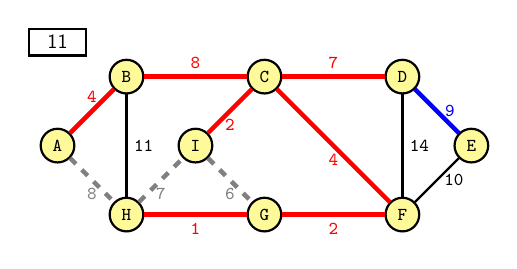
\begin{tikzpicture}[
	scale=0.73, 
	transform shape,
	thick,
	font=\ttfamily\bfseries\small
]
\tikzset{
    mynode/.style = {circle, draw=black, align=center,fill=yellow!40},
    edgen/.style = {-},
    edger/.style = {-,ultra thick,red},
    edgeb/.style = {-,ultra thick,blue},
    edgegg/.style = {-,ultra thick,gray,dashed},
}
\node[rectangle,draw=black,font=\sffamily, minimum width=1cm] at (0.0,3.0) {11};
\node[mynode] at (0.0,1.2) (a) {A};
\node[mynode] at (1.2,2.4) (b) {B};
\node[mynode] at (6.0,2.4) (d) {D};
\node[mynode] at (3.6,2.4) (c) {C};
\node[mynode] at (1.2,0.0) (h) {H};
\node[mynode] at (3.6,0.0) (g) {G};
\node[mynode] at (6.0,0.0) (f) {F};
\node[mynode] at (2.4,1.2) (i) {I};
\node[mynode] at (7.2,1.2) (e) {E};
%
\draw[edger] (a) edge node[above] {4} (b);
\draw[edger] (b) edge node[above] {8} (c);
\draw[edger] (c) edge node[above] {7} (d);
\draw[edgeb] (d) edge node[above,right] {9} (e);
%
\draw[edgegg] (a) edge node[below] {8} (h);
\draw[edger] (h) edge node[below] {1} (g);
\draw[edger] (g) edge node[below] {2} (f);
\draw[edgen] (f) edge node[below,right] {10} (e);
%
\draw[edgegg] (h) edge node[below] {7} (i);
\draw[edgegg] (i) edge node[below] {6} (g);
\draw[edger] (i) edge node[below] {2} (c);
%
\draw[edgen] (b) edge node[right] {11} (h);
\draw[edgen] (d) edge node[right] {14} (f);
\draw[edger] (c) edge node[below] {4} (f);
\end{tikzpicture}	
\hfill
%%%%%% 12 %%%%%%%%%%%%%%%%%
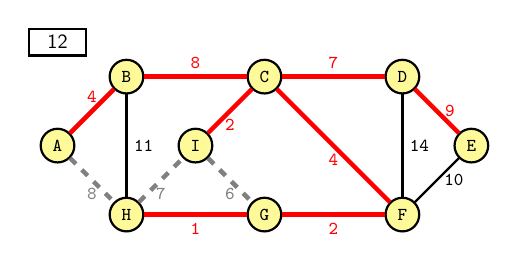
\begin{tikzpicture}[
	scale=0.73, 
	transform shape,
	thick,
	font=\ttfamily\bfseries\small
]
\tikzset{
    mynode/.style = {circle, draw=black, align=center,fill=yellow!40},
    edgen/.style = {-},
    edger/.style = {-,ultra thick,red},
    edgeb/.style = {-,ultra thick,blue},
    edgegg/.style = {-,ultra thick,gray,dashed},
}
\node[rectangle,draw=black,font=\sffamily, minimum width=1cm] at (0.0,3.0) {12};
\node[mynode] at (0.0,1.2) (a) {A};
\node[mynode] at (1.2,2.4) (b) {B};
\node[mynode] at (6.0,2.4) (d) {D};
\node[mynode] at (3.6,2.4) (c) {C};
\node[mynode] at (1.2,0.0) (h) {H};
\node[mynode] at (3.6,0.0) (g) {G};
\node[mynode] at (6.0,0.0) (f) {F};
\node[mynode] at (2.4,1.2) (i) {I};
\node[mynode] at (7.2,1.2) (e) {E};
%
\draw[edger] (a) edge node[above] {4} (b);
\draw[edger] (b) edge node[above] {8} (c);
\draw[edger] (c) edge node[above] {7} (d);
\draw[edger] (d) edge node[above,right] {9} (e);
%
\draw[edgegg] (a) edge node[below] {8} (h);
\draw[edger] (h) edge node[below] {1} (g);
\draw[edger] (g) edge node[below] {2} (f);
\draw[edgen] (f) edge node[below,right] {10} (e);
%
\draw[edgegg] (h) edge node[below] {7} (i);
\draw[edgegg] (i) edge node[below] {6} (g);
\draw[edger] (i) edge node[below] {2} (c);
%
\draw[edgen] (b) edge node[right] {11} (h);
\draw[edgen] (d) edge node[right] {14} (f);
\draw[edger] (c) edge node[below] {4} (f);
\end{tikzpicture}	

\end{frame}



%-------------------------------------------------------------------------
\begin{frame}{Analisi della complessità algoritmo di Kruskal}

\BIL
\item Il tempo di esecuzione per l’algoritmo di Kruskal dipende dalla realizzazione della struttura dati per Merge-Find Set
\item Utilizziamo la versione con \alert{euristica sul rango + compressione},\\ (*) le cui operazioni hanno costo ammortizzato costante 

\medskip
\begin{tabular}{|l|l|l|}
\hline
\textbf{Fase} & \textbf{Volte} & \textbf{Costo} \\\hline
Inizializzazione & 1 & $O(n)$ \\\hline
Ordinamento & 1 & $O(m \log m)$ \\\hline
Operazioni \textsf{find}(),\textsf{merge}() & $O(m)$ & $O(1)^{(*)}$ \\\hline
\end{tabular}
\item Totale:  $O(n + m \log m + m) = O(m \log m) = O(m \log n^2) = O(m \log n)$
\EIL
\end{frame}

%-------------------------------------------------------------------------
\begin{frame}{Algoritmo di Prim}


\vspace{-9pt}
\begin{myboxtitle}[Idea]
\BIL
\item L’algoritmo di Prim procede mantenendo in A un singolo albero 
\item L’albero parte da un vertice arbitrario $r$ (la radice) e cresce fino a quando non ricopre tutti i vertici
\item Ad ogni passo viene aggiunto un arco leggero che collega un vertice in $V_A$ con un vertice in $V-V_A$,
dove $V_A$ è l'insieme di nodi raggiunti da archi in $A$
\EIL
\end{myboxtitle}

\begin{myboxtitle}[Correttezza]
\BIL
\item $(V_A,V-V_A)$ è un taglio che rispetta $A$ (per definizione)
\item Per il corollario, gli archi leggeri che attraversano il taglio sono sicuri
\EIL
\end{myboxtitle}

\end{frame}

%-------------------------------------------------------------------------
\begin{frame}{Implementazione}

\vspace{-9pt}
\begin{myboxtitle}[Struttura dati per i nodi non ancora nell'albero]
\BI
\item Durante l'esecuzione, i vertici non ancora nell'albero si trovano in una 
coda con min-priorità $Q$ ordinata in base alla seguente definizione di priorità
\item "La priorità del nodo $v$ è il peso minimo di un arco che collega $v$ ad
un vertice nell'albero, o $+\infty$ se tale arco non esiste"
\EI
\end{myboxtitle}

\begin{myboxtitle}[Albero registrato come \alert{vettore dei padri}]
\BI
\item Ogni nodo $v$ mantiene un puntatore al padre $p[v]$
\item $A$ è mantenuto implicitamente: $A = \{ (v, p[v]) ~|~ v \in V - Q - \{ r \} \}$
\EI
\end{myboxtitle}

\end{frame}



%-------------------------------------------------------------------------
\begin{frame}[shrink=10]{Algoritmo di Prim}

\vspace{-12pt}
\begin{Procedure}
\caption[A]{$\INTARRAY\ \prim(\Graph\ G,\ \Node\ r)$}

$\Heap\ Q = \minheapconstructor()$\;
$\PriorityItem[\,]\ \Pos = \NEW\ \PriorityItem[1 \mldots G.n]$\;
$\INTARRAY\ p = \NEW\ \INTEGER[1 \mldots G.n]$\;
\ForEach{$u \in G.\VV() - \{ r \}$}{
  $\Pos[u] = Q.\heapinsert(u, +\infty)$\;
}
$\Pos[r] = Q.\heapinsert(r, 0)$\;
$p[r] = 0$\;
\While{\NOT $\ Q.\setempty()$}{
  $\Node\ u = Q.\heapdeletemin()$\;
  $\Pos[u] = \Nil$\;
  \ForEach{$v \in G.\adj(u)$}{
    \If{$\Pos[v] \neq \Nil$ \AND\ $w(u,v) < \Pos[v].\mathit{priority}$}{
      $Q.\heapdecrease(\Pos[v], w(u,v))$\;
      $p[v] = u$\;
    }
  }
}
\Return $p$\;
\end{Procedure}
\end{frame}

%-------------------------------------------------------------------------
\begin{frame}{Esempio}
%%%%%% 1 %%%%%%%%%%%%%%%%%
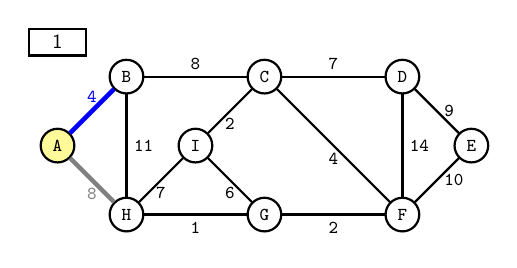
\begin{tikzpicture}[
	scale=0.73, 
	transform shape,
	thick,
	font=\ttfamily\bfseries\small
]
\tikzset{
    mynode/.style = {circle, draw=black, align=center,fill=white},
    mynodeb/.style = {circle, draw=black, align=center,fill=yellow!40},
    edgen/.style = {-},
    edger/.style = {-,ultra thick,red},
    edgeb/.style = {-,ultra thick,blue},
    edgeg/.style = {-,ultra thick,gray},
}
\node[rectangle,draw=black,font=\sffamily, minimum width=1cm] at (0.0,3.0) {1};
\node[mynodeb] at (0.0,1.2) (a) {A};
\node[mynode] at (1.2,2.4) (b) {B};
\node[mynode] at (6.0,2.4) (d) {D};
\node[mynode] at (3.6,2.4) (c) {C};
\node[mynode] at (1.2,0.0) (h) {H};
\node[mynode] at (3.6,0.0) (g) {G};
\node[mynode] at (6.0,0.0) (f) {F};
\node[mynode] at (2.4,1.2) (i) {I};
\node[mynode] at (7.2,1.2) (e) {E};
%
\draw[edgeb] (a) edge node[above] {4} (b);
\draw[edgen] (b) edge node[above] {8} (c);
\draw[edgen] (c) edge node[above] {7} (d);
\draw[edgen] (d) edge node[above,right] {9} (e);
%
\draw[edgeg] (a) edge node[below] {8} (h);
\draw[edgen] (h) edge node[below] {1} (g);
\draw[edgen] (g) edge node[below] {2} (f);
\draw[edgen] (f) edge node[below,right] {10} (e);
%
\draw[edgen] (h) edge node[below] {7} (i);
\draw[edgen] (i) edge node[below] {6} (g);
\draw[edgen] (i) edge node[below] {2} (c);
%
\draw[edgen] (b) edge node[right] {11} (h);
\draw[edgen] (d) edge node[right] {14} (f);
\draw[edgen] (c) edge node[below] {4} (f);
\end{tikzpicture}
\hfill
%%%%%% 2 %%%%%%%%%%%%%%%%%
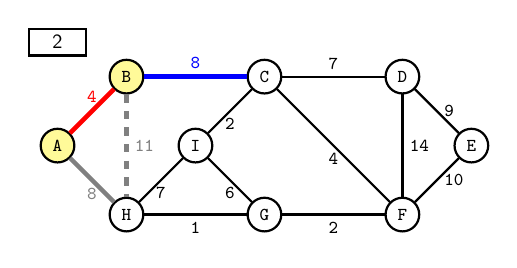
\begin{tikzpicture}[
	scale=0.73, 
	transform shape,
	thick,
	font=\ttfamily\bfseries\small
]
\tikzset{
    mynode/.style = {circle, draw=black, align=center,fill=white},
    mynodeb/.style = {circle, draw=black, align=center,fill=yellow!40},
    edgen/.style = {-},
    edger/.style = {-,ultra thick,red},
    edgeb/.style = {-,ultra thick,blue},
    edgeg/.style = {-,ultra thick,gray},
    edgegg/.style = {-,ultra thick,gray,dashed},
}
\node[rectangle,draw=black,font=\sffamily, minimum width=1cm] at (0.0,3.0) {2};
\node[mynodeb] at (0.0,1.2) (a) {A};
\node[mynodeb] at (1.2,2.4) (b) {B};
\node[mynode] at (6.0,2.4) (d) {D};
\node[mynode] at (3.6,2.4) (c) {C};
\node[mynode] at (1.2,0.0) (h) {H};
\node[mynode] at (3.6,0.0) (g) {G};
\node[mynode] at (6.0,0.0) (f) {F};
\node[mynode] at (2.4,1.2) (i) {I};
\node[mynode] at (7.2,1.2) (e) {E};
%
\draw[edger] (a) edge node[above] {4} (b);
\draw[edgeb] (b) edge node[above] {8} (c);
\draw[edgen] (c) edge node[above] {7} (d);
\draw[edgen] (d) edge node[above,right] {9} (e);
%
\draw[edgeg] (a) edge node[below] {8} (h);
\draw[edgen] (h) edge node[below] {1} (g);
\draw[edgen] (g) edge node[below] {2} (f);
\draw[edgen] (f) edge node[below,right] {10} (e);
%
\draw[edgen] (h) edge node[below] {7} (i);
\draw[edgen] (i) edge node[below] {6} (g);
\draw[edgen] (i) edge node[below] {2} (c);
%
\draw[edgegg] (b) edge node[right] {11} (h);
\draw[edgen] (d) edge node[right] {14} (f);
\draw[edgen] (c) edge node[below] {4} (f);
\end{tikzpicture}

\bigskip
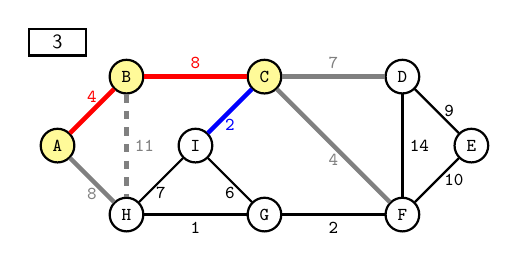
\begin{tikzpicture}[
	scale=0.73, 
	transform shape,
	thick,
	font=\ttfamily\bfseries\small
]
\tikzset{
    mynode/.style = {circle, draw=black, align=center,fill=white},
    mynodeb/.style = {circle, draw=black, align=center,fill=yellow!40},
    edgen/.style = {-},
    edger/.style = {-,ultra thick,red},
    edgeb/.style = {-,ultra thick,blue},
    edgeg/.style = {-,ultra thick,gray},
    edgegg/.style = {-,ultra thick,gray,dashed},
}
\node[rectangle,draw=black,font=\sffamily, minimum width=1cm] at (0.0,3.0) {3};
\node[mynodeb] at (0.0,1.2) (a) {A};
\node[mynodeb] at (1.2,2.4) (b) {B};
\node[mynode] at (6.0,2.4) (d) {D};
\node[mynodeb] at (3.6,2.4) (c) {C};
\node[mynode] at (1.2,0.0) (h) {H};
\node[mynode] at (3.6,0.0) (g) {G};
\node[mynode] at (6.0,0.0) (f) {F};
\node[mynode] at (2.4,1.2) (i) {I};
\node[mynode] at (7.2,1.2) (e) {E};
%
\draw[edger] (a) edge node[above] {4} (b);
\draw[edger] (b) edge node[above] {8} (c);
\draw[edgeg] (c) edge node[above] {7} (d);
\draw[edgen] (d) edge node[above,right] {9} (e);
%
\draw[edgeg] (a) edge node[below] {8} (h);
\draw[edgen] (h) edge node[below] {1} (g);
\draw[edgen] (g) edge node[below] {2} (f);
\draw[edgen] (f) edge node[below,right] {10} (e);
%
\draw[edgen] (h) edge node[below] {7} (i);
\draw[edgen] (i) edge node[below] {6} (g);
\draw[edgeb] (i) edge node[below] {2} (c);
%
\draw[edgegg] (b) edge node[right] {11} (h);
\draw[edgen] (d) edge node[right] {14} (f);
\draw[edgeg] (c) edge node[below] {4} (f);
\end{tikzpicture}
\hfill
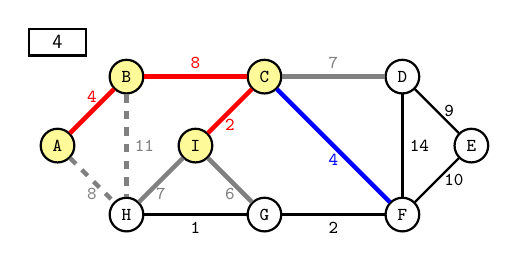
\begin{tikzpicture}[
	scale=0.73, 
	transform shape,
	thick,
	font=\ttfamily\bfseries\small
]
\tikzset{
    mynode/.style = {circle, draw=black, align=center,fill=white},
    mynodeb/.style = {circle, draw=black, align=center,fill=yellow!40},
    edgen/.style = {-},
    edger/.style = {-,ultra thick,red},
    edgeb/.style = {-,ultra thick,blue},
    edgeg/.style = {-,ultra thick,gray},
    edgegg/.style = {-,ultra thick,gray,dashed},
}
\node[rectangle,draw=black,font=\sffamily, minimum width=1cm] at (0.0,3.0) {4};
\node[mynodeb] at (0.0,1.2) (a) {A};
\node[mynodeb] at (1.2,2.4) (b) {B};
\node[mynode] at (6.0,2.4) (d) {D};
\node[mynodeb] at (3.6,2.4) (c) {C};
\node[mynode] at (1.2,0.0) (h) {H};
\node[mynode] at (3.6,0.0) (g) {G};
\node[mynode] at (6.0,0.0) (f) {F};
\node[mynodeb] at (2.4,1.2) (i) {I};
\node[mynode] at (7.2,1.2) (e) {E};
%
\draw[edger] (a) edge node[above] {4} (b);
\draw[edger] (b) edge node[above] {8} (c);
\draw[edgeg] (c) edge node[above] {7} (d);
\draw[edgen] (d) edge node[above,right] {9} (e);
%
\draw[edgegg] (a) edge node[below] {8} (h);
\draw[edgen] (h) edge node[below] {1} (g);
\draw[edgen] (g) edge node[below] {2} (f);
\draw[edgen] (f) edge node[below,right] {10} (e);
%
\draw[edgeg] (h) edge node[below] {7} (i);
\draw[edgeg] (i) edge node[below] {6} (g);
\draw[edger] (i) edge node[below] {2} (c);
%
\draw[edgegg] (b) edge node[right] {11} (h);
\draw[edgen] (d) edge node[right] {14} (f);
\draw[edgeb] (c) edge node[below] {4} (f);
\end{tikzpicture}

\end{frame}

%-------------------------------------------------------------------------
\begin{frame}{Esempio}

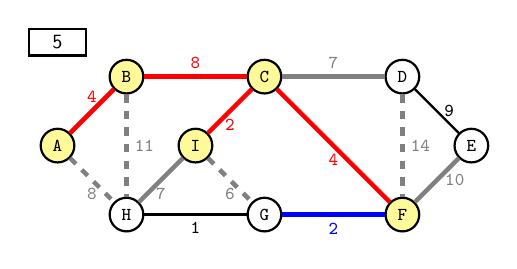
\begin{tikzpicture}[
	scale=0.73, 
	transform shape,
	thick,
	font=\ttfamily\bfseries\small
]
\tikzset{
    mynode/.style = {circle, draw=black, align=center,fill=white},
    mynodeb/.style = {circle, draw=black, align=center,fill=yellow!40},
    edgen/.style = {-},
    edger/.style = {-,ultra thick,red},
    edgeb/.style = {-,ultra thick,blue},
    edgeg/.style = {-,ultra thick,gray},
    edgegg/.style = {-,ultra thick,gray,dashed},
}
\node[rectangle,draw=black,font=\sffamily, minimum width=1cm] at (0.0,3.0) {5};
\node[mynodeb] at (0.0,1.2) (a) {A};
\node[mynodeb] at (1.2,2.4) (b) {B};
\node[mynode] at (6.0,2.4) (d) {D};
\node[mynodeb] at (3.6,2.4) (c) {C};
\node[mynode] at (1.2,0.0) (h) {H};
\node[mynode] at (3.6,0.0) (g) {G};
\node[mynodeb] at (6.0,0.0) (f) {F};
\node[mynodeb] at (2.4,1.2) (i) {I};
\node[mynode] at (7.2,1.2) (e) {E};
%
\draw[edger] (a) edge node[above] {4} (b);
\draw[edger] (b) edge node[above] {8} (c);
\draw[edgeg] (c) edge node[above] {7} (d);
\draw[edgen] (d) edge node[above,right] {9} (e);
%
\draw[edgegg] (a) edge node[below] {8} (h);
\draw[edgen] (h) edge node[below] {1} (g);
\draw[edgeb] (g) edge node[below] {2} (f);
\draw[edgeg] (f) edge node[below,right] {10} (e);
%
\draw[edgeg] (h) edge node[below] {7} (i);
\draw[edgegg] (i) edge node[below] {6} (g);
\draw[edger] (i) edge node[below] {2} (c);
%
\draw[edgegg] (b) edge node[right] {11} (h);
\draw[edgegg] (d) edge node[right] {14} (f);
\draw[edger] (c) edge node[below] {4} (f);
\end{tikzpicture}
\hfill
\begin{tikzpicture}[
	scale=0.73, 
	transform shape,
	thick,
	font=\ttfamily\bfseries\small
]
\tikzset{
    mynode/.style = {circle, draw=black, align=center,fill=white},
    mynodeb/.style = {circle, draw=black, align=center,fill=yellow!40},
    edgen/.style = {-},
    edger/.style = {-,ultra thick,red},
    edgeb/.style = {-,ultra thick,blue},
    edgeg/.style = {-,ultra thick,gray},
    edgegg/.style = {-,ultra thick,gray,dashed},
}
\node[rectangle,draw=black,font=\sffamily, minimum width=1cm] at (0.0,3.0) {6};
\node[mynodeb] at (0.0,1.2) (a) {A};
\node[mynodeb] at (1.2,2.4) (b) {B};
\node[mynode] at (6.0,2.4) (d) {D};
\node[mynodeb] at (3.6,2.4) (c) {C};
\node[mynode] at (1.2,0.0) (h) {H};
\node[mynodeb] at (3.6,0.0) (g) {G};
\node[mynodeb] at (6.0,0.0) (f) {F};
\node[mynodeb] at (2.4,1.2) (i) {I};
\node[mynode] at (7.2,1.2) (e) {E};
%
\draw[edger] (a) edge node[above] {4} (b);
\draw[edger] (b) edge node[above] {8} (c);
\draw[edgeg] (c) edge node[above] {7} (d);
\draw[edgen] (d) edge node[above,right] {9} (e);
%
\draw[edgegg] (a) edge node[below] {8} (h);
\draw[edgeb] (h) edge node[below] {1} (g);
\draw[edger] (g) edge node[below] {2} (f);
\draw[edgeg] (f) edge node[below,right] {10} (e);
%
\draw[edgegg] (h) edge node[below] {7} (i);
\draw[edgegg] (i) edge node[below] {6} (g);
\draw[edger] (i) edge node[below] {2} (c);
%
\draw[edgegg] (b) edge node[right] {11} (h);
\draw[edgegg] (d) edge node[right] {14} (f);
\draw[edger] (c) edge node[below] {4} (f);
\end{tikzpicture}

\bigskip
\begin{tikzpicture}[
	scale=0.73, 
	transform shape,
	thick,
	font=\ttfamily\bfseries\small
]
\tikzset{
    mynode/.style = {circle, draw=black, align=center,fill=white},
    mynodeb/.style = {circle, draw=black, align=center,fill=yellow!40},
    edgen/.style = {-},
    edger/.style = {-,ultra thick,red},
    edgeb/.style = {-,ultra thick,blue},
    edgeg/.style = {-,ultra thick,gray},
    edgegg/.style = {-,ultra thick,gray,dashed},
}
\node[rectangle,draw=black,font=\sffamily, minimum width=1cm] at (0.0,3.0) {7};
\node[mynodeb] at (0.0,1.2) (a) {A};
\node[mynodeb] at (1.2,2.4) (b) {B};
\node[mynode] at (6.0,2.4) (d) {D};
\node[mynodeb] at (3.6,2.4) (c) {C};
\node[mynodeb] at (1.2,0.0) (h) {H};
\node[mynodeb] at (3.6,0.0) (g) {G};
\node[mynodeb] at (6.0,0.0) (f) {F};
\node[mynodeb] at (2.4,1.2) (i) {I};
\node[mynode] at (7.2,1.2) (e) {E};
%
\draw[edger] (a) edge node[above] {4} (b);
\draw[edger] (b) edge node[above] {8} (c);
\draw[edgeb] (c) edge node[above] {7} (d);
\draw[edgen] (d) edge node[above,right] {9} (e);
%
\draw[edgegg] (a) edge node[below] {8} (h);
\draw[edger] (h) edge node[below] {1} (g);
\draw[edger] (g) edge node[below] {2} (f);
\draw[edgeg] (f) edge node[below,right] {10} (e);
%
\draw[edgegg] (h) edge node[below] {7} (i);
\draw[edgegg] (i) edge node[below] {6} (g);
\draw[edger] (i) edge node[below] {2} (c);
%
\draw[edgegg] (b) edge node[right] {11} (h);
\draw[edgegg] (d) edge node[right] {14} (f);
\draw[edger] (c) edge node[below] {4} (f);
\end{tikzpicture}
\hfill
\begin{tikzpicture}[
	scale=0.73, 
	transform shape,
	thick,
	font=\ttfamily\bfseries\small
]
\tikzset{
    mynode/.style = {circle, draw=black, align=center,fill=white},
    mynodeb/.style = {circle, draw=black, align=center,fill=yellow!40},
    edgen/.style = {-},
    edger/.style = {-,ultra thick,red},
    edgeb/.style = {-,ultra thick,blue},
    edgeg/.style = {-,ultra thick,gray},
    edgegg/.style = {-,ultra thick,gray,dashed},
}
\node[rectangle,draw=black,font=\sffamily, minimum width=1cm] at (0.0,3.0) {8};
\node[mynodeb] at (0.0,1.2) (a) {A};
\node[mynodeb] at (1.2,2.4) (b) {B};
\node[mynodeb] at (6.0,2.4) (d) {D};
\node[mynodeb] at (3.6,2.4) (c) {C};
\node[mynodeb] at (1.2,0.0) (h) {H};
\node[mynodeb] at (3.6,0.0) (g) {G};
\node[mynodeb] at (6.0,0.0) (f) {F};
\node[mynodeb] at (2.4,1.2) (i) {I};
\node[mynode] at (7.2,1.2) (e) {E};
%
\draw[edger] (a) edge node[above] {4} (b);
\draw[edger] (b) edge node[above] {8} (c);
\draw[edger] (c) edge node[above] {7} (d);
\draw[edgeb] (d) edge node[above,right] {9} (e);
%
\draw[edgegg] (a) edge node[below] {8} (h);
\draw[edger] (h) edge node[below] {1} (g);
\draw[edger] (g) edge node[below] {2} (f);
\draw[edgegg] (f) edge node[below,right] {10} (e);
%
\draw[edgegg] (h) edge node[below] {7} (i);
\draw[edgegg] (i) edge node[below] {6} (g);
\draw[edger] (i) edge node[below] {2} (c);
%
\draw[edgegg] (b) edge node[right] {11} (h);
\draw[edgegg] (d) edge node[right] {14} (f);
\draw[edger] (c) edge node[below] {4} (f);
\end{tikzpicture}


\end{frame}

%-------------------------------------------------------------------------
\begin{frame}{Esempio}
\centering
\begin{tikzpicture}[
	scale=1.2, 
	transform shape,
	thick,
	font=\ttfamily\bfseries\small
]
\tikzset{
    mynode/.style = {circle, draw=black, align=center,fill=white},
    mynodeb/.style = {circle, draw=black, align=center,fill=yellow!40},
    edgen/.style = {-},
    edger/.style = {-,ultra thick,red},
    edgeb/.style = {-,ultra thick,blue},
    edgeg/.style = {-,ultra thick,gray},
    edgegg/.style = {-,ultra thick,gray,dashed},
}
\node[rectangle,draw=black,font=\sffamily, minimum width=1cm] at (0.0,3.0) {9};
\node[mynodeb] at (0.0,1.2) (a) {A};
\node[mynodeb] at (1.2,2.4) (b) {B};
\node[mynodeb] at (6.0,2.4) (d) {D};
\node[mynodeb] at (3.6,2.4) (c) {C};
\node[mynodeb] at (1.2,0.0) (h) {H};
\node[mynodeb] at (3.6,0.0) (g) {G};
\node[mynodeb] at (6.0,0.0) (f) {F};
\node[mynodeb] at (2.4,1.2) (i) {I};
\node[mynode] at (7.2,1.2) (e) {E};
%
\draw[edger] (a) edge node[above] {4} (b);
\draw[edger] (b) edge node[above] {8} (c);
\draw[edger] (c) edge node[above] {7} (d);
\draw[edger] (d) edge node[above,right] {9} (e);
%
\draw[edgegg] (a) edge node[below] {8} (h);
\draw[edger] (h) edge node[below] {1} (g);
\draw[edger] (g) edge node[below] {2} (f);
\draw[edgegg] (f) edge node[below,right] {10} (e);
%
\draw[edgegg] (h) edge node[below] {7} (i);
\draw[edgegg] (i) edge node[below] {6} (g);
\draw[edger] (i) edge node[below] {2} (c);
%
\draw[edgegg] (b) edge node[right] {11} (h);
\draw[edgegg] (d) edge node[right] {14} (f);
\draw[edger] (c) edge node[below] {4} (f);
\end{tikzpicture}
\end{frame}


%-------------------------------------------------------------------------
\begin{frame}{Algoritmo di Prim: Analisi}

L’efficienza dell’algoritmo di Prim dipende dalla coda con priorità

\BIL
\item Se si utilizza uno \alert{heap binario}:

\bigskip
\begin{tabular}{|l|l|l|}
\hline
\textbf{Fase} & \textbf{Volte} & \textbf{Costo} \\\hline
Inizializzazione & 1 & $O(n \log n)$ \\\hline
$\textsf{deleteMin}()$ & $O(n)$ & $O(\log n)$ \\\hline
$\textsf{decreasePriority}()$ & $O(m)$ & $O(\log n)$ \\\hline
\end{tabular}

\bigskip
Tempo totale: \alert{$O(n+n \log n + m \log n)=O(m \log n)$}, asintoticamente uguale a quello di Kruskal.
\item Cosa succede se la coda con priorità è implementata tramite \alert{vettore non ordinato}?
\EIL
\end{frame}

%-------------------------------------------------------------------------
\begin{frame}{Discussione}

\vspace{-9pt}
\begin{myboxtitle}[Vero o falso]
\BI
\item L’arco con peso minimo è sicuro
\item L’arco con il secondo peso minimo è sicuro
\item L’arco con il terzo peso minimo è sicuro
\EI
\end{myboxtitle}

\begin{myboxtitle}[Albero di copertura minima in un piano]
\BI
\item Input: $n$ punti nel piano 
\item Il peso di una coppia di punti è dato dalla distanza euclidea fra di essi
\item Trovare un insieme di connessioni di peso minimo
\item Da non confondere con gli \alert{Steiner tree}
\EI
\end{myboxtitle}

\end{frame}

%-------------------------------------------------------------------------
\begin{frame}{Applicazioni}

\vspace{-9pt}
\begin{myboxtitle}[Applicazioni dirette per la progettazione]
\BI
\item Reti di telecomunicazione
\item Reti idriche
\item Reti di trasporto
\item Reti elettriche
\EI
\end{myboxtitle}

\begin{myboxtitle}[Alcuni utilizzi particolari]
\BI
\item Segmentazione di immagini
\item Riconoscimento scrittura manuale
\item Disegno di circuiti elettronici
\item Progettazione tassonomie
\EI
\end{myboxtitle}

\end{frame}


%-------------------------------------------------------------------------
\begin{frame}{Prospettiva storica}
	
\BIL
\item \alert{$O(m \log n)$}:
	\BI
	\item Primo algoritmo: Boruvka (1926)
	\item Kruskal (1956)
	\item Prim (1957), ma anche Jarnik (1930)
	\EI
\item \alert{$O(m + n \log n)$}:
	\BI
	\item Fredman-Tarjan (1987)
	\item Modifica di Prim che utilizza gli heap di Fibonacci
	\EI
\item \alert{$O(m+n)$}:	
	\BI
	\item Algoritmo probabilistico di Karger, Klein, Tarjan (1995)
	\item Vari algoritmi in tempo lineare per casi particolari
	\item Questione aperta se si possa risolvere il problema in tempo
	  lineare deterministico
	\EI
\EIL

	
\end{frame}



%-------------------------------------------------------------------------
\begin{frame}{Conclusioni}

\vspace{-9pt}
\begin{myboxtitle}[Vantaggi]
\BIL
\item Semplici da programmare
\item Molto efficienti
\item Quando è possibile dimostrare la proprietà di scelta ingorda, danno la soluzione ottima
\item La soluzione sub-ottima può essere accettabile
\EIL
\end{myboxtitle}

\begin{myboxtitle}[Svantaggi]
\BIL
\item Non sempre applicabili se si vuole la soluzione ottima
\EIL
\end{myboxtitle}

\end{frame}


\end{document}



